% ------------------------------------------------------------------------
% ------------------------------------------------------------------------
% ICMC: Modelo de Trabalho Acadêmico (tese de doutorado, dissertação de
% mestrado e trabalhos monográficos em geral) em conformidade com 
% ABNT NBR 14724:2011: Informação e documentação - Trabalhos acadêmicos -
% Apresentação
% ------------------------------------------------------------------------
% ------------------------------------------------------------------------

% Opções: 
%   Qualificação         = qualificacao 
%   Curso                = doutorado/mestrado
%   Situação do trabalho = pre-defesa/pos-defesa (exceto para qualificação)
% -- opções do pacote babel --
% Idioma padrão = brazil
	%spanish,			% idioma adicional para hifenização
	%english,			% idioma adicional para hifenização
	%brazil				% o último idioma é o principal do documento
\documentclass[doutorado, pre-defesa, brazil, english]{packages/icmc}

% ---
% Pacotes Opcionais
% ---
\usepackage{rotating}           % Usado para rotacionar o texto
\usepackage[all,knot,arc,import,poly]{xy}   % Pacote para desenhos gráficos
% Este pacote pode conflitar com outros pacotes gráficos como o ``pictex''
% Então é necessário usar apenas um dos pacotes conflitantes


%---------------------------------
%pacotes que eu adicionei
%---------------------------------
\usepackage{todonotes}
\usepackage{xcolor}

% acronyms
\usepackage{acronym}

\usepackage{lipsum}

%---------------------------------
%pacotes que eu adicionei - FIM
%---------------------------------

\usepackage{multirow}
\usepackage{booktabs}
\usepackage{adjustbox}
\usepackage{hyperref}

\newcommand{\VerbL}{0.52\textwidth}
\newcommand{\LatL}{0.42\textwidth}

% Comando simples para exibir comandos Latex no texto
\newcommand{\comando}[1]{\textbf{$\backslash$#1}}
\newcommand\myworries[1]{\textcolor{red}{#1}}

% ---
% Informações de dados para CAPA e FOLHA DE ROSTO
% ---
% Keywords: Harnessing Gamification Techniques to Cope with Learner’s Motivation 
% Persuasion technology, persuasion profiling
\titulo{ "to do" ... on Constraint-Based Group Formation}
\autor[Borges, S. de S.]{Simone de Sousa Borges}
\orientador[Advisor]{Prof. Dr.}{Seiji Isotani}

\curso{CCMC}
\data{3}{4}{2017} % Data do depósito
% ---


% ---
% RESUMOS
% ---

% Resumo em português
% conter no máximo 500 palavras
\textoresumo{
    Este trabalho é ... 
    
    }{Gamificação, Techonologia Persuasiva, Aprendizagem Colaborativa com Suporte Computacional }

% ---
% resumo em inglês
% ---
\textoresumo[english]{
    This study ...
    group formation in CSCL refers to the process of adequately select and group students together to create scenarios and situations that help the learning process to occur more efficiently and smoothly. When groups are created randomly or without careful considerations, collaborative learning may provoke inefficient interactions that compromise the learning process and the motivation of students. Thus, throughout the years, several studies have been investigating group formation initiatives in collaborative learning environments based on computational and pedagogical criteria.
    }{Gamification, Persuasive Technology, Computer-Supported Collaborative Learning}
   
    
% ---
% Configurações de aparência do PDF final
% ---
% alterando o aspecto da cor azul
\definecolor{blue}{RGB}{41,5,195}

% informações do PDF
\makeatletter
\hypersetup{
     	pagebackref=true,
		pdftitle={\@title}, 
		pdfauthor={\@author},
    	pdfsubject={\imprimirpreambulo},
	    pdfcreator={LaTeX with abnTeX2/ICMC-USP},
		pdfkeywords={\palavraschave}, 
		colorlinks=true,       		% false: boxed links; true: colored links
    	linkcolor=blue,          	% color of internal links
    	citecolor=blue,        		% color of links to bibliography
    	filecolor=magenta,      	% color of file links
		urlcolor=blue,
		bookmarksdepth=4
}
\makeatother
% --- 

% ----------------------------------------------------------
% ELEMENTOS PRÉ-TEXTUAIS
% ----------------------------------------------------------

% Inserir a ficha catalográfica
%\incluifichacatalografica*{tex/fichaCatalografica.pdf}
\incluifichacatalografica{634} % Código Cutter: número atribuído ao sobrenome do autor. Para obtê-lo, consulte a tabela Cutter Sanborn (em http://www.davignon.qc.ca/cutter1.html), procure pelo sobrenome ou forma mais próxima ao sobrenome completo e coloque o número indicado como parâmetro.


% DEDICATÓRIA / AGRADECIMENTO / EPÍGRAFE
\textodedicatoria*{tex/pre-textual/dedicatoria}
\textoagradecimentos*{tex/pre-textual/agradecimentos}
\textoepigrafe*{tex/pre-textual/epigrafe}

% Inclui a lista de figuras
\incluilistadefiguras

% Inclui a lista de tabelas
\incluilistadetabelas

% Inclui a lista de quadros
\incluilistadequadros

% Inclui a lista de algoritmos
\incluilistadealgoritmos

% Inclui a lista de códigos
\incluilistadecodigos

% Inclui a lista de siglas e abreviaturas
\incluilistadesiglas

% Inclui a lista de símbolos
\incluilistadesimbolos

% ----
% Início do documento
% ----
\begin{document}
% ----------------------------------------------------------
% ELEMENTOS TEXTUAIS
% ----------------------------------------------------------
\textual

\chapter{Introduction}
\label{chapter:introducao}
\section{Context}

\sigla{CL}{Collaborative learning} has been around for quite some time, but recently it gained prominence because of advances in computer technology (e.g., popularization of laptops, tablets, and smart phones) and the widespread use of Internet-based educational tools (e.g., \sigla{LMSs}{Learning menagement systems} and \sigla{MOOCs}{Massive Open Online Courses}) \cite{From_mirroring_to_guiding}.
As pointed out by \citeonline{CSCL_historical_perspective}, Internet has brought up renewed interest in investigating the benefits of computer support when applied to CL.
These advances have set the stage for Computer-Supported Collaborative Learning (CSCL), which is a pedagogical strategy where individuals study in groups, and knowledge is constructed through discussions, argumentation, exchange of ideas, conflict resolution, and so on \cite{CSCL_historical_perspective}. 
In such pedagogical strategy, computers play a key role in supporting the learning process by making feasible the design, orchestration and assessment of group activities in several different contexts and situations \cite{CSCL_and_Innovation}.
Many studies have been investigating the benefits of CSCL \cite{CSCL_historical_perspective,Collaborative_Learning_Techniques,Theory-Driven_Group_Formation,Designing_for_interaction}. 
According to the community's findings, collaboration has a positive influence on the learning process, mainly when it is well designed and properly applied \cite{The_pedagogical_challenges_to_collaborative_technologies}. 
Thus, CSCL environments and CL activities should be carefully designed; otherwise, there is no guarantee that the learning results will meet students’ goals or teachers’ expectations \cite{Why_some_groups_fail,Collaborative_Learning_Techniques}. 

Research efforts in CSCL are concentrated on the development of technologies to support the creation of \textit{situations} where people can \textit{interact} with each other, and as a desirable outcome, triggering \textit{learning mechanism} that can positively \textit{influence learning outcomes} \cite{What_do_you_mean_by}. 
The creation of computational systems to support CSCL demands a deep understanding of many concepts, among them one of the most important is the group formation process \cite{An_ontology_engineering_approach}. 
Group formation is an umbrella term that covers several strategies, algorithms, techniques, and methods to cluster individuals according to several criteria \cite{Group_Formation_Algorithms}. 
Considering free collaboration does not produces systematic learning outcomes \cite{An_ontology_engineering_approach}, group formation plays a fundamental role in CSCL since it influences how students perceive the environment, interact with peers, use available didactic materials, and take part in learning activities \cite{Over-scripting_CSCL}. 
The main objective of  group formation is the creation of well-thought-out groups that will lead students to better interact with each other, thus maximizing the potential of better learning gains \cite{Designing_for_interaction,Collaborative_Learning_Techniques}. 
Groups can be formed based on learners similar interests, needs, and competences; or, quite the opposite, groups can be based, for example, on complementary competences, however with common purposes \cite{Specifying_computer_supported_collaboration_scripts}. 

Unlike teacher-fronted learning sessions (i.e., where teacher can control the interactions), the success of online group work is highly influenced by learners willingness to participate \cite{Causal_Relationships_Between}. 
However, several factors may interfere on such willingness. For instance, as pointed out in \cite{Gamification_of_Collaborative_Learning}, when scripts designed to support CL tasks are used, there are situations in which  these scripts can interfere with students’ motivation. 
% --------------------------------------------------------------------
% citar no cap de CSCL exemplos de situations e quais estou resolvendo
% --------------------------------------------------------------------
The interplay of motivation and cognition when students undertake collaborative group work is a research area that has not been fully investigated \cite{The_interrelationship_of_emotion_and_cognition}. 
Still, it can be a promising area, because the success of both individual and group learning is closely related to the motivation of the students \cite{Computer_supported_team_based_learning}. 
There are numerous different motivation construct analyses in the literature \cite{Self-determination_theory_and_the_facilitation}.
Usually, these analyses share a common distinction between two topics: intrinsic and extrinsic motivation. Briefly, extrinsic motivators are external factors to the person that can influence his/her interest and attitudes, while intrinsic motivation is related to internal mental states able to trigger person’s predisposition towards interests and attitudes \cite{Beyond_Talk_Creating_Autonomous_Motivation}.

Among other solutions, researchers and practitioners have been investigating how gamification-based alternatives can be used to motivate students in learning scenarios \cite{kapp2012gamification,A_systematic_mapping,Does_Gamification_Work}.
However, since gamification is highly context-dependent, ill-designed gamification solutions can lead to harmful effects instead of the expected benefits \cite{Demographic_differences_in_perceived_benefits,The_Bright_and_Dark_Sides_of_Gamification}. 
Moreover, few efforts have tried to investigate how to design appropriate gamified activities (e.g., environment’s design), meaningful rewards (e.g., suitable game elements), and proper players’ roles to positively influence learner's willingness to participate in group work \cite{A_Link_Between_Worlds}. 
%Ler intro do Seiji, organizar esta ultima parte de forma similar

% -----------------------------------------------------
% Problem Delimitation
% -----------------------------------------------------
\section{Problem Delimitation}
Most group formation strategies found in the literature are focused on learner's cognitive dimension (learning path) as learning style and competences, for instance, while the motivational dimension (psychological path) has grabbed less attention (Appendix \ref{chapter:gf_mapping}). 
This research suggests that gamification is one of the persuasive technology strategies that can capitalize on group formation support. We followed the threefold formula proposed by~\cite{the_craft_of_research} to flesh out the scope of this research:\footnote{
\citeonline{the_craft_of_research} refer to research problem as \emph{practical} or \emph{conceptual problem} and potential contribution as \emph{significance}.
}
\begin{itemize}
\item Research Problem
\end{itemize}
Group formation when imposed can influence learners' needs for autonomy, therefore impacting their willingness to join groups.

\begin{itemize}
\item Research Questions (RQs):
	\begin{itemize}
	\item RQ1: Can gamification be harnessed to support constraint-based group formation?
    \item RQ2: Can gamification influence learners' willingness to join groups?
	\end{itemize}
\end{itemize}

\begin{itemize}
\item Potential Contributions
\end{itemize}

% -----------------------------------------------------
% Motivation
% -----------------------------------------------------
\section{Motivation}
\begin{comment}
FRANCESA
The lack of psychological aspects in usual current User Models and Profiles has motivated this
Thesis. Nowadays profiles with personal psychological details are not the main concern for web
system designers and programmers. Some research has been made by Affective Computing
scientists focusing mainly on the identification and modelling of user’s Emotions [RHR98],
[OCC88], [Ort02], [Lis02], [ZC03], [Pic00], [Pic97], [Pic02], [LTC+00], [Ell92], [Pai00].
Recently, studies from [Dam94], [Dam99], [Sim83], [Gol95], [Pai00], [Pic97], [Pic00], [Pic02],
[TPP03], [Tha06] have demonstrated how important psychological aspects of people such as
Personality Traits and Emotions are during the human decision-making process. Human Emotion and their models have already been largely implemented in computers, much more than Personality 

VINA
Testing tools are usually built on top of HLL VMs. As a result, they often end up tampering with the emergent computation. Usually, the additional layers between the program
under test and the underlying HLL VM introduced by testing tools can have a pernicious
effect on the emergent computation. Furthermore, during run time, when tools need to
carry out computations about themselves (or the program under test) they must turn
to costly metaprogramming operations (e.g., reflection). To examine a running program,
for example, a tool has to perform introspection operations (i.e., inspecting state and
structure). Likewise, to change the behavior or structure of the program under test during
run time, tools have to resort to intercession (Lee and Zachary, 1995).
Apart from the overhead incurred by reflective operations, tools that implement weak
mutation rely heavily on state storage and retrieval. By storing state information these
tools factor out the expense of running all mutants from the beginning. Nevertheless, such
computational savings are only possible at the expense of a significantly larger memory
footprint (Fleyshgakker and Weiss, 1994).
\end{comment}

% -----------------------------------------------------
% Specific Objectives and Rationale
% -----------------------------------------------------
\section{Specific Objectives and Rationale}
\begin{comment}
\textit{The objective of this research is to investigate whether XXX are a
cost-effective technology for supporting software testing. Towards this end, we set out
to extend the infrastructure provided by a JIT-enabled JVM with software testing support.
The rationale behind arguing that HLL VMs provide a sound basis for building an
integrated mutation testing environment is that they bear a repertoire of runtime data
structures suitable for accommodating the semantics of mutation testing. First, by capitalizing on existing runtime structures it is possible to decrease the amount of storage
space required to implement weak mutation: from within the execution environment it is
easier to determine what needs to be copied, narrowing the scope down and thus reducing
storage requirements. Second, there is no need to resort to costly reflective operations since
runtime information are readily available at HLL VM level. Third, by reifying mutation
analysis concepts (i.e., turning them into first-class citizens within the scope of HLL VMs)
it is easier to take advantage of high-end optimization and memory management features
7Chapter 1 | Introduction
which are common in mainstream HLL VM implementations, e.g., just-in-time (JIT) compilation and garbage collection (GC). Lastly, a further advantage of building on HLL VMs
data structures is that they make it possible to exert greater control over the execution of
mutants.
As stated, the inherent non-determinism of concurrent programs makes software testing
and debugging even more challenging. Therefore, a key missing element in modern execution environments is the ability to deterministically re-execute multithreaded programs.
Since HLL VMs are the locus of control during execution, we conjecture that these execution environments contain facilities that can be extended to prune away non-deterministic
behavior and enforce that subsequent executions cover distinct thread schedules from the
ones previously run.
The rationale behind settling on using a JVM realization to implement our VM-based
mutation analysis environment is that, apart from being by far the most used HLL VM
implementation within academic circles (Durelli et al., 2010), implementations of such
execution environment have sophisticated, built-in multithread support. This makes for
an infrastructure more suited to our integrated software testing environment because both
the fork-and-join model to speed up mutants execution and the deterministic replayer
heavily rely on thread support.}
\end{comment}

\subsection{Non Objectives}

propose a new compilation of game elements, instead we investigated 

In this thesis,we do not aim to propose another list of game design elements. Instead, our goal is to investigate whether the effects of a subset of game design elements (a subset that is not exhaustive) regularly discussed in the literature, can harness learner's psychological needs in a constraint-based group formation approach.



% -----------------------------------------------------
% Conventions Used Throughout this PhD Dissertation
% -----------------------------------------------------
\section{Conventions Used Throughout this PhD Dissertation}


% -----------------------------------------------------
% Structure of this PhD Dissertation
% -----------------------------------------------------
\section{Structure of this PhD Dissertation}










\chapter{Computer-Supported Collaborative Learning}
\label{chapter:background-cscl}
\label{cha:background-cscl}
In Chapter \ref{chapter:introducao}, we briefly introduced some aspects of Computer-Supported Collaborative Learning (CSCL). In this chapter will provide a better overview on CSCL background. Firstly, we will present some considerations about CSCL and related topics, as intentional design, CSCL scripts, and interaction patterns, for instance. Secondly, we will provide an overview of the efforts the CSCL community has been doing to improve group formation (GF). More specifically, We are concerned with how groups have been created, what criteria to cluster learners in groups have been most investigated, and what are the rationale behind the selection of such criteria. Finally, in the last section we will make some considerations.

There are several definitions and/or related concepts around collaborative learning (CL) in the literature. In this thesis, the term collaborative learning is used to refer to students working in intentionally designed groups. We are aware that there are situations where teachers ask students to form groups and work together freely, however, free collaboration does not necessarily leads to learning gains \cite{An_Ontological_Engineering_Approach_tese}, and several researchers have already reported that ill-designed CL activities can lead to unsuccessful group learning \cite{Motivation_in_a_computer-supported_collaborative_learning}. CL benefits can be enhanced when technological support is provided. So, CSCl is a pedagogical approach that can foster learning by providing to the learners situations to study in groups. In such approach, computers are tools that support the learning process and social interactions \cite{CSCL_historical_perspective}. 

Current research on CSCL have investigated how to scaffold learners interactions, 


Learning as a consequence of the planned 

So to be effective means, ...

\section{CSCL Scripts}

\section{Interaction Patterns}

\subsection{Interaction Patterns based on Collaborative Learning Techniques}

\subsection{Interaction Patterns based on Learning Theories}

\section{Group Formation}
There are several denominations for the act of grouping learners in the context of collaborative learning, such as, group/team composition (Hsu et al. 2008) group or team formation (Yannibelli and Amandi 2012), grouping students (Alfonseca et al. 2006), clustering students (Chiu and Hsiao 2010). Basically, these denominations have the same meaning, as the act of bringing together students in effective learning groups (Isotani et al. 2009). In this work, we adopt the term group formation, which is the most widely term used in the investigated studies.
Although the term "effective" can have different meanings among researchers, in this field is often used as a synonym for the proper allocation of resources to enhance the learning process (Isotani et al. 2009). These resources can be tangible (e.g. learning materials and tools to support collaboration) or intangible (e.g. knowledge and skills to be learned). Most research on group formation have focused on how to allocate these resources based on the learners profiles, on the technologies involved, or on the tasks to be performed (CL techniques, also knows as CL best practices) (Magnisalis et al. 2011).

Using learners' profiles helps instructors adequately deliver custom content to satisfy, not only individual necessities of the learners, but also group's necessities (Alfonseca et al. 2006; Faria et al. 2006; Greer et al. 1998; Ounnas et al. 2009; Graf and Bekele 2006), while inputs from the environment, can give more information that can help to understand the collaborative context and as a result, to improve grouping quality (Muehlenbrock 2005; Villasclaras-Fernández et al. 2009; Hernández-Leo et al. 2011; Wesner and Pfister 2001) . Finally, there are other approaches for group formation that relies on using specifications of CL techniques to acquire sufficient information to group the learners (Isotani et al. 2009).

Generally, the formation of groups can be performed randomly (e.g. assigning learners in the groups by chance), self-selected (i.e. the learners choose with whom they want to study), or it can be carried out by an instructor or computing system, based on some criteria (Ikeda and Mizoguchi 1997; Alfonseca et al 2006; Graf and Bekele 2006; Hsu and Chou 2008; Ounnas et al. 2009; Boticki et al. 2013; Greer et al. 1998; Faria et al. 2006)
As discussed by (Dillenbourg and Jermann 2007) and (Laurillard 2009), the benefits of collaborative learning arise only when there is a detailed and proper planning of components and collaborative mechanisms. Considering these, many authors have raised concerns regard random selection and self-selected approaches since these approaches can result in unequal participation such as, students in the same group working at a different pace, off-task behavior, or even increasing students’ resistance to group work (Barkley et al. 2005; Dillenbourg 2002; Isotani and Mizoguchi 2008; ). Moreover, one way to increase the chances of forming groups more capable to achieve the desired learning goals is assigning learners to groups using approaches based on CL techniques (Barkley et al. 2005; Dillenbourg 2002; Stahl 2004; Isotani et al. 2009).

Regardless of the strategy used, the research in the area sought to investigate ways to influence positively the behavior of individuals to form groups where their presence and that of their peers are relevant; that interactions are significant; and to maximize the chances that knowledge construction will occur in more favorable conditions. 

%-------------------------------------------------------
% Concluding Remarks
%-------------------------------------------------------
\section{Concluding Remarks}



\chapter{Gamification}
\label{chapter:gamification}
%-------------------------------------------------------
% Gamification Techniques
%-------------------------------------------------------

Gamification consists of using game developing techniques in
non-game environments, such as social networks [16], e-health, e-commerce, and educational systems. The techniques and resources used in digital games have elements
capable of (i) motivate users,(i) hold their interest, and (iii) challenge them
to solve problems. In gamification approaches, these elements are
not the center of the system, instead these elements have the purpose of attract users and motivate them to keeping using it [28]. Foursquare application (Figure 1-b) is an
example of a gamified system. Foursquare is a location-based
social network, which reached one billion “check-ins” in 2011 [ref].
Foursquare allows users to check-in at venues using a device specific
front-end to the application (e.g., mobile website), each
check-in might award the user with user-points or “badges”. 
\textit{Explicar pointification, 
Argumentar que evoluiu agora trend personalização.}

% Gamification
\begin{figure}[h!]
\caption{Foursquare screens, from left to right, list of user's check-ins and badges earned. }
\centering
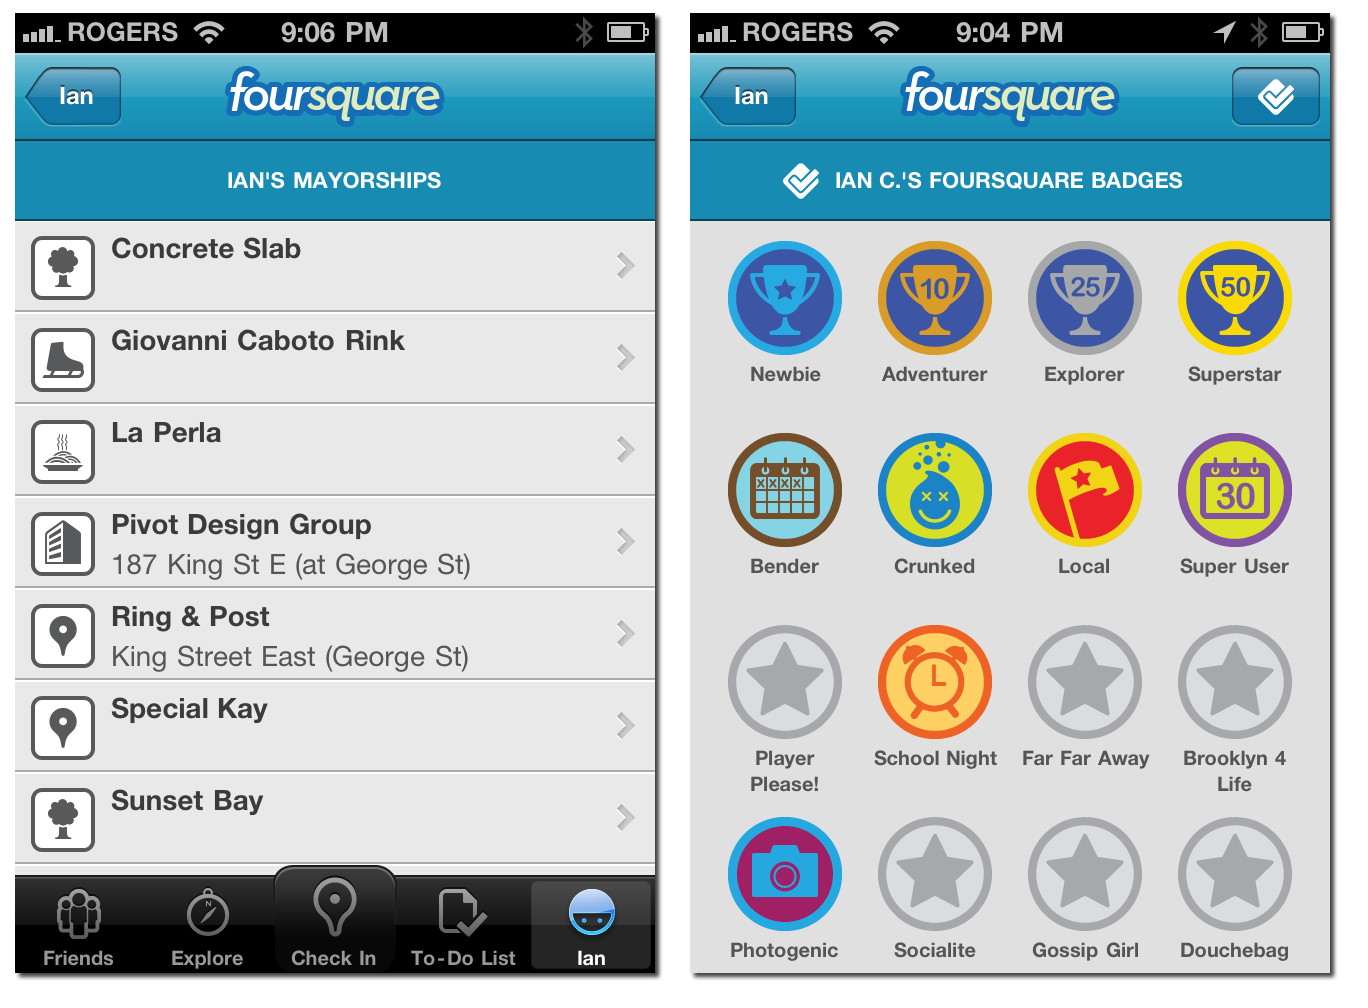
\includegraphics[width=0.4\textwidth]{foursquare}
\label{fig:foursquere}
\end{figure}

\textbf{What Gamification is not}

Here, we will define some concepts related to the term "game". The following discussion is not comprehensive, and it is only intended to clarify and narrow down our definition of gamification. A more comprehensive and deep discussion can be found in \citeauthor{Deterding2011}.

\begin{itemize}
\item Gamification is not Playful design or gameful design:
\end{itemize}

Playful design is using game-based aesthetics or limited usability
based on game elements in non-game contexts with the purpose of
drawing the user's attention [1]. These elements are used to amuse
users and cause an emotional response. One successful example is
Twitter’s page knows as “Fail Whale” (Figure 1-a). Whenever
there is an overload on the servers, instead of a boring page with
some standard error message, users are presented with a drawing of
a dozen birds, twitters, trying to lift a whale.

% Playful design or gameful design
\begin{figure}[h!]
\caption{“Fail Whale”, a playful illustration of the "503 Service Unavailable" status}
\centering

\includegraphics[width=0.4\textwidth]{failwhale}
\label{fig:failwhale}
\end{figure}

\begin{itemize}
\item Gamification is not Serious games:
\end{itemize}

Serious games are games designed for non-recreational
environments and for educational purposes [16]. The term
“serious” is employed because these games can focus on areas as
diverse as economics, education, health, industry, military,
engineering, and politics. In environments created by applying
serious game concepts, it is possible to simulate real-world
situations without incurring in eventual costs and risks. The main
goal of this sort of training-environment is to convey information
to the user [31]. The Virtual Incident Management Training System
(Figure 1-c) is a multiplayer training environment designed for
training professionals that need to act swiftly in case of accident on
highways, such as paramedics and policemen [37].

% Serious game
\begin{figure}[h!]
\caption{The Virtual Incident Management Training System initial screen. Source: \cite{catt_lab2017}}
\centering
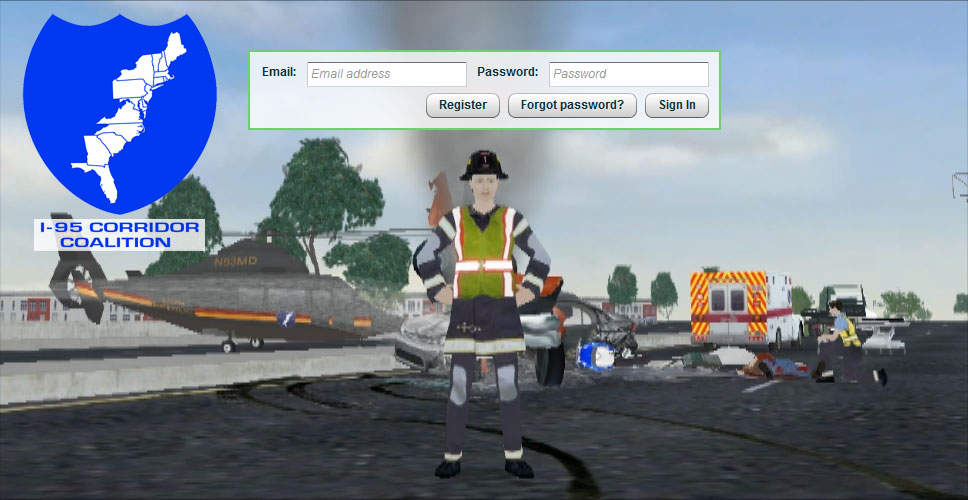
\includegraphics[width=0.5\textwidth]{serious_games}
\label{fig:serious_games}
\end{figure}

\begin{itemize}
\item Gamification is not Video games or digital games:
\end{itemize}

Video Games or Digital Games are systems in which users are
engaged in resolving abstract conflicts and challenges, under
predetermined rules [36]. In this scenario the game continuously
offers interactivity and feedback to the user, which often result in
an emotional reaction. Figure 1-d shows a screenshot of the game
New Super Mario Bros.Wii\copyright whose main character, Mario, is
considered one of the most iconic video game characters.

% Video games or Digital games
\begin{figure}[h!]
\caption{New Super Mario Bros.wii a game developed and publishid by Nintendo}
\centering
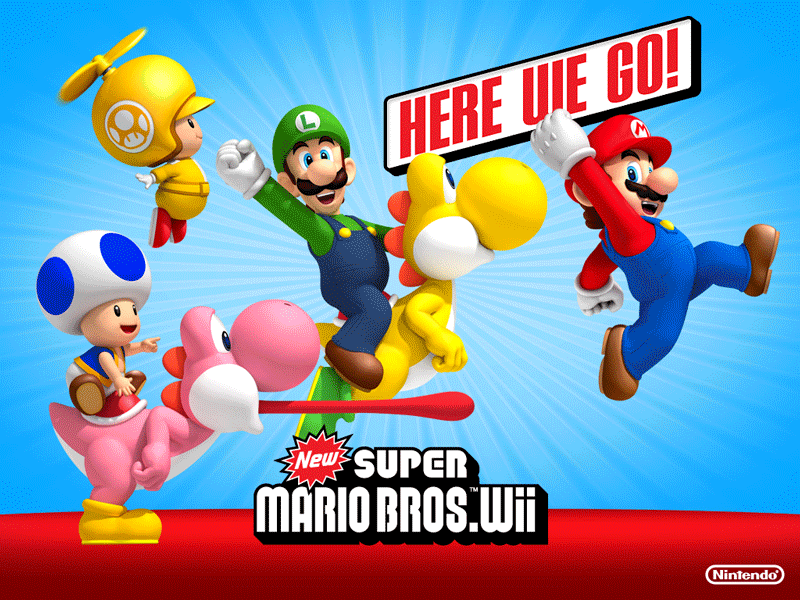
\includegraphics[width=0.4\textwidth]{super_mariowii}
\label{fig:super_mariowii}
\end{figure}

It is worth to point out that the current thesis focus on covering
research that explicitly match our definition of Gamification.
Therefore, we are not considering research based on serious games,
video games, playful design and other uses of game concepts in
educational contexts.

%-------------------------------------------------------
% Game Design Elements
%-------------------------------------------------------
\section{Game Design Elements}
\label{sec:Game_Design_Elements}

\sigla{GDE}{Game design elements} is a term used to cover a broad list of game mechanics, dynamics, and aesthetics used in the design and development of games \cite{kapp2012gamification,Gamification_of_Collaborative_Learning}. In the gamification process, these elements work as motivational \textit{affordances} to deliver gameful experiences to the users, and as a consequence, trying to influence their behavior \cite{Does_Gamification_Work}. 
A high-level definition of GDE categories, usually found in the literature, is as it follows: 

\begin{itemize}
\item \textbf{Mechanics} They define the rules, actions and behaviors allowed in the game, and they are characterized by game components at the level of data representation and algorithms:
\subitem Examples: Rules, goals (objectives), levels, number of players. 
\item \textbf{Dynamics} characterize the run-time behavior of the mechanics reacting on player inputs;
\subitem Examples: Feedback, conflict, competition, cooperation, time pressure.
\item \textbf{Aesthetics} characterize the interaction with the game system (i.e., input-output and vice versa).
\subitem Examples: Sensation, fantasy, narrative, challenge, fellowship, discovery, expression.
\end{itemize}

According to \citeauthor{hunicke2004}, starting from the designer’s perspective,
the mechanics rise the dynamic system behavior, which in turn produces aesthetic experiences that will be consumed by the player.
However, from the player’s perspective, aesthetics set the \textit{tone} of the experience as a direct result of player's reaction to the dynamics, in turn, dynamics are paced by the available mechanics. For this reason it is important to have both perspectives in focus, and neglecting none of them.

% Video games or Digital games
\begin{figure}[h!]
\caption{Designers and players have different, but linked, perspectives of the game. Adapted from \cite{hunicke2004}}
\centering
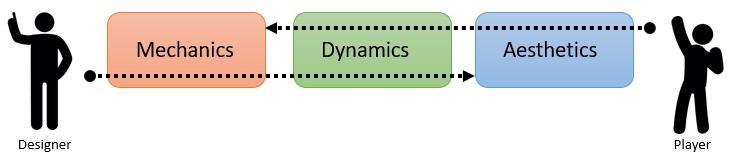
\includegraphics[width=0.8\textwidth]{mda_views}
\label{fig:mda_views}
\end{figure}

To illustrate how game elements can be linked, we will provide an example of scenario using the game element \textbf{Challenge}. Challenge is an example of aesthetic element, and it is a powerful one since it poises an obstacle between the player and the reward/victory. 
For instance, challenge can be created by the dynamic \textbf{time pressure}, where the player has limited time to accomplish a task. 
In turn, time pressure to exist depends of mechanics such as \textbf{rules specification} (e.g., how much time does the player have?) and \textbf{rules implementation} (e.g., algorithms and data). 
As an usage example of such approach, we can cite the Super Mario Bros \textsuperscript{\textregistered} game franchise. In many games of the franchise, the character Mario needs to reach the end of the stage before running out of time otherwise, the player will fail the challenge (Figure \ref{fig:mda}). Figure \ref{fig:duolingo} shows an example of the same usage, challenge based on time pressure, however in a non-game application. The application in question is Duolingo, a well known free language-learning platform. Duolingo is a successful example of how gamification can be skillfully applied to a system \cite{Huynh2016}. In the example, the learner needs to complete a task in an specific amount of time to be rewarded. 
% https://www.quora.com/How-effective-is-Duolingo-in-learning-a-language
% Figura Mario
\begin{figure}[h!]
\caption{Usage example of "challenge based on time pressure" in a game.}
\centering
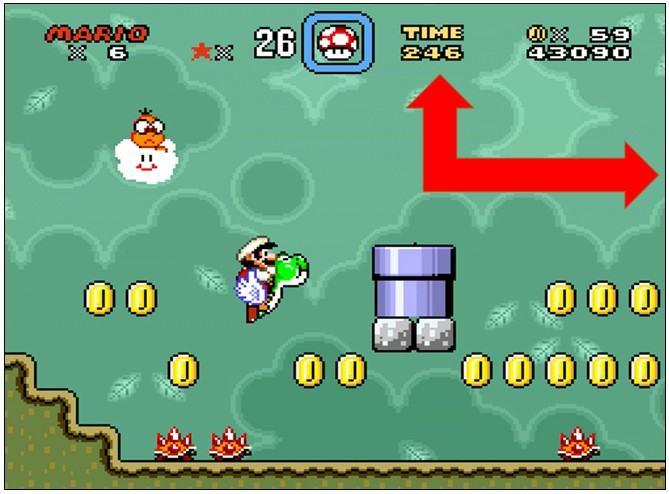
\includegraphics[width=0.4\textwidth]{mda}
\label{fig:mda}
\end{figure}

% Figura Duolingo
\begin{figure}[h!]
\caption{Usage example of "challenge based on time pressure" in a gamified application.}
\centering
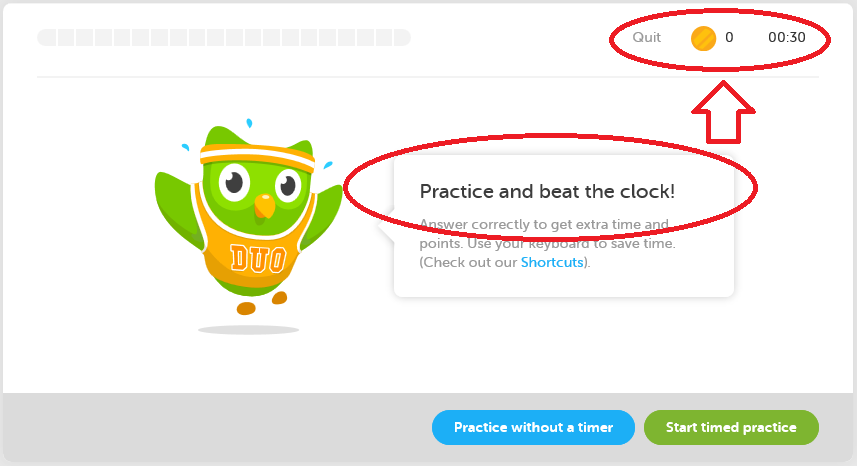
\includegraphics[width=0.6\textwidth]{duolingo2}
\label{fig:duolingo}
\end{figure}

GDE have been exhaustedly discussed in the gamification literature \cite{kapp2012gamification,robinson2013preliminary,werbach2012win,zichermann2010game,zichermann2011gamification,Ferro2013}.
Many researchers have tried to summarize these elements and create a unified taxonomy. However, up to this point, there is no consensus about an universal compilation. 
For this reason, 
there are several lists, conceptual frameworks, and guidelines with compilations of game design elements in the literature \cite{Ferro2013,A_Link_Between_Worlds}. 
Regardless the overlaps or parallels found in these lists, 
they can great differ from one to another making the design and implementation of gamification techniques harder \cite{Sailer2017}.

In this thesis, it is not our intention to propose a new compilation of game elements. So, we will stick with the game design elements shown in Table X . Although it is not an extensive compilation, all these elements have been extensively used in the game industry (i.e., best practices) \cite{ferro2016gamification}, and have been empirically evaluated in many gamification studies\cite{Sailer2017}. In addition, we will not try to explain the overlaps and relationships between each and all elements shown in Table 1. Instead, we are more interested in investigate how the selected game design elements can be harnessed to support constraint-based group formation.

Table 

%-------------------------------------------------------
% Player Types
%-------------------------------------------------------
\section{Player Typologies}
\label{sec:Player_Typologies}

The concept of player types is based on the assumption that different persons have different reactions given a certain game element \cite{fullerton2008}.
One of the first player typologies used in gamification was Bartle's Player Types \footnote{Richard Bartle created the model, the so called "Bartle's Player Test" was later implemented by Erwin Andreasen and Brandon Downey \cite{Bartle2009}}. However, since the publication of Bartle's seminal study, several other models have been proposed. In this section an overview of some important typologies in the context of this thesis is provided. 

\subsection{Bartle's Players Types}
\label{sec:Bartle_Players_Types}

Richard Bartle co-created a text-based game called \sigla{MUD}{Multi-User Dungeon}, the ancestor of today's \sigla{MMORPGs}{Massively Multiplayer Online Role-Playing Games}. 
He performed some observations in the game environment trying to figure out what players were looking for in the game (i.e., MUD). 
By analyzing the answers of a questionnaire and from observing players behaviors within the game, he conceived four player psychological portraits in a MUD: Killers, Achievers, Explorers and Socializers \cite{Bartle1996}. 
The taxonomy provided by \citeauthor{Bartle1996} are the foundations of player types research, but it has its limitations. 
For instance, Bartle's model was constructed using comparisons between scenarios that respondents must choose. 
As pointed by \citeauthor{yee2006motivations}, if a questionnaire has questions that force the respondent to choose between two scenarios, the answer may represent a dichotomy, and bias may occur towards various outcomes.
In addition, as explained by \citeauthor{Bartle2009}, the model was created to fulfill a different purpose and it was never intended to be used in the gamification domain.
For instance, \citeauthor{youtube_bartle} alert that the model might be incomplete for other domains than MUD's and as a consequence, designers might be "forced" to fit players in some available category  (i.e., therefore ignoring their personal traits) or even ignore "non-recognized" players types (i.e., players that do not "fit" any available types) \cite{Bartle2009}.


\subsection{BrainHex}
\label{sec:BrainHex}

According to \cite{bateman2011player}, the creation of robust and efficient player models need be rooted on trait theory of players preferences. 
Nevertheless, while research on psychometric typology for personality has a long history, player typology and trait theories of play are still in their infancy. 
BrainHex is a player satisfaction model build on previous efforts from the  \sigla{DGD1}{first Demographic Game Design model} and the \sigla{DGD2}{second Demographic Game Design model} \cite{Nacke2014}. 
BrainHex build up on insights from neurobiological findings from these models and presents seven different archetypes of players: Seeker, Survivor, Daredevil, Mastermind, Conqueror, Socialiser, and Achiever. These archetypes are related to typologies such as Myers-Briggs \cite{myers1985manual}, and each one characterizes a specific player type.
The model was validated using data collected from a survey and comparing the demographic data to different BrainHex archetypes. Using the results of the psychometric orientation of respondents, they established a relationships between personality types and BrainHex archetypes. Data was collected from 50,000 respondents.

\subsection{Motivations for Playing Online}
\label{sec:motivations_for_playing_online}

Bartle's work was conducted in a exploratory fashion, however without the support of more robust statistical analysis \cite{yee2006motivations}. In the research conducted by \citeauthor{yee2006motivations}, a compilation of suitable motivations for playing in MMORPGs was created based on the literature (i.e., Bartle’s Player Types) and open-ended responses from several surveys. Using these information, a unified Likert-type survey was created. The surveys target audience was MMORPGs players. Data from 3200 respondents was collected and \sigla{FA}{factor analysis} was used to investigate the survey answers. At the beginning, 10 factors were extracted, and after performing another analysis of these 10 factors, three main factors were identified: Achievement, Social and Immersion. A summary of these results is shown in Table~\ref{tab:motivations_for_play_yee}.

% Please add the following required packages to your document preamble:
% \usepackage{booktabs}
\begin{table}[]
\centering
\caption{Main components of motivations to play in MMORPGs \cite{yee2006motivations}}
\label{tab:motivations_for_play_yee}
\begin{tabular}{@{}llc@{}}
\toprule
\textbf{Main Component} & \textbf{Subcomponent} & \multicolumn{1}{l}{\textbf{Factor Loading}} \\ \midrule
\textbf{Achievement} & Advancement & 0.85 \\
 & Mechanics & 0.77 \\
 & Competition & 0.68 \\
\textbf{Social} & Socializing & 0.74 \\
 & Relantionship & 0.62 \\
 & Teamwork & 0.76 \\
\textbf{Immersion} & Discovery & 0.72 \\
 & Role-Play & 0.70 \\
 & Customization & 0.66 \\
 & Escapism & 0.53 \\ \bottomrule
\end{tabular}
\end{table}

Motivations to Play \cite{yee2006motivations} has its roots on Bartle's model, but it differs from the original one in many points. 
The main difference between Yee's and Bartle's models is that instead of four main player types, \citeauthor{yee2006motivations} identified three main motivational components.
In addition, this three components are composed of subcomponents.
At the end, the model proposed by \citeauthor{yee2006motivations} does not attempt to identify in which archetype one player fits but rather to understand a set of components and how much each component can influence the player. 
By identifying the reasons that may arouse motivation to play, and by analyzing the results of the scoring system developed, one can also identify what can be deemed less attractive for such an individual. 

%-------------------------------------------------------
% Gamification Applied to Education
%-------------------------------------------------------
\section{Gamification Applied to Education}

Students motivation can play a vital role in students academic performance and achievements since it can influence the amount of effort and time spent in learning activities \cite{linehan2011}. So, there is a growing interest in gamification as well as its applications and implications in the field of education. This growing interest is mainly due to the potential of gamification techniques to motivate students during the process of learning \cite{Borges2014SAC}.
However, gamification has been used in education with mixed results \cite{Berkling2013,Does_Gamification_Work,Mekler2015,Lieberoth2015,Dichev2017}. 
Some empirical findings indicate that gamification can increase motivation and engagement in students; other findings highlight that gamification can be a distraction to students; and therefore it may end up hindering learning. 

In 2013, we carried out a systematic mapping study of research into gamification applied to education trying to identify studies covering and classifying the types of research being published and the most investigated topics in the area \cite{Borges2014SAC}. Using this systematic method it is possible to aggregate and categorize primary studies, creating an overview of the research area in question \cite{petersen2008}. 

At first, we ran some searches using a combination of candidate keywords. These trial searches combined the keyword \textbf{gamification} with some synonyms related to \textbf{education} and \textbf{learning}. No limit of publication date was used (i.e., data range). Even though, due to the  small number of papers returned from the resulting strings, we decided that only the keyword \textbf{gamification} should be used. Later, by applying predefined inclusion  criteria, we manually selected only research in the education field. 
These decisions allowed us to analyze a greater number of papers, lowering the odds of leaving relevant studies out of our final set. Using gamification as keyword, we performed searches on electronic databases that are known to cover relevant scientific journals and articles from a wide variety of domains such as Computer Science, Education and Educational Research, Science, Engineering, Medicine and Psychology. Initially, we retrieved 357 primary papers. However, only 48 candidate papers were obtained after applying the inclusion and exclusion criteria based upon title and abstract. Finally, after going over introductions and conclusions, we ended up with a final set of 26 primary papers as shown in Table~\ref{tab:visao_geral_busca}. In this section we will summarize the main results of the literature review, but Appendix~\ref{chapter:gf_mapping} contains the rationale that backs up the literature review, statistics performed, and a list of selected papers in first version.


\begin{table}
[ht] \caption {Papers retrieved from each electronic database, total of candidate studies, and the final set.} \label{tab:visao_geral_busca} 
	\begin{center}
		\begin{tabular}
			{ | l | c | c |} 
				\hline\hline   & \textbf{Jun/2013} & \textbf{Fev/2017} \\
                \hline \textbf{ACM Digital Library} & 144 & 451 \\
				\hline \textbf{IEEE Xxplore} & 31 & 490 \\
				\hline \textbf{Elsevier (via Science Direct)} & 32 & 1210 \\
				\hline \textbf{Springer} & 55 & 109\\
                \hline \textbf{SCOPUS} & 95 & 4741\tablefootnote{Results already retrieved from the databases above were not excluded, as we did in 2013.} \\
			\hline \hline \textsc{\textbf{Total}} & 357 & 7001\\
			\hline \textbf{Candidates} & 48 & -\\
			\hline \textbf{Final set} & 26 & -\\
			\hline\hline 
		\end{tabular}
	\end{center}
\end{table}



%-------------------------------------------------------
% Gamification in CSCL
%-------------------------------------------------------
\subsection{Gamification in CSCL}

To deal with this problem, it is necessary to design gamification to fit properly in individual and collaborative learning contexts. Unfortunately, there is a lack of studies on frameworks mapping game elements and learning theories to support the adequate design and application of gamification in education. 


There is a large amount of research on motivation and learning coming from different background; all demonstrating that motivation plays a vital role for individual learning. However, in the case of CSCL, learning is a more complex process, and despite this, research in this field has not been completely explored yet \cite{Motivation_in_a_computer-supported_collaborative_learning}. In [16] for instance, a meta-analysis of 41 studies investigated the effects of having choice (re-lated to autonomy) and possible intrinsic motivation outcomes. These studies investigated both children and adults samples in different environments. The meta-analysis shows evidence that backs up the idea that enabling learners to choose from different learning alternatives enhanced not only intrinsic motivation, but also: task performance, effort, and perceived competence. However, in [9], they raised some concerns regards trying to manipulate students’ motivation. In this study, an experiment was performed and students' competence was evaluated (if appropriate) after completing specific collaborative tasks. The exploratory analyses presented evidences that the appraisal of one partner’s may have played an unexpected role increasing a free-riding behavior on students that did not received an appraisal. The authors assumed that the free-riding effect indicates that part of the participants lost their motivation, thus suggesting the influence of motivation also during CSCL. 




\chapter{Persuasive Technology}
\label{chapter:persuasive-techonology}
%-------------------------------------------------------
% The Persuasive Technology Theory
%-------------------------------------------------------
\section{The Persuasive Technology Theory}
\lipsum[1]

%-------------------------------------------------------
% Persuasion Profiling
%-------------------------------------------------------
\section{Persuasion Profiling}

Persuasive technology is an approach that intends to change user’s attitudes and/or behavior using persuasion [1]. Persuasive technology feasibility has increased thanks to recent computing advances and the surge of interest in the area. Evidence that persuasive technologies can persuade users can be found in [2]–[6]. In intelligent learning environments, persuasive technologies have been used to increase students’ engagement and to reduce the feeling of obligation towards executing pedagogical tasks [7]. However, as pointed out by [8], a reliable use of persuasion strategies involves delivering the right message in a specific way at the precise moment. Yet, trying to figure out what is “the right message” for a student and how to deliver it at the “right time” are still difficult tasks. 
As shown in [9] and in [10], the design and implementation of persuasive (learning) systems are complex tasks since it is hard to estimate the effectiveness of those strategies regarding each learner. As stated by [11], many social psychologists have pointed out that one sound way to improve the effectiveness of persuasive attempts relies on the design of personalized persuasive strategies, tailored to fit user’s personality traits. Thus, we can design the “right message”, and deliver it at the “right time” to the “right user”. Nevertheless, most research still focus on the target benefits that can be achieved using persuasive systems, and less research have been found on how to design effective approaches tailored to different users in order reach such benefits [2], [3], [12]. Significant contributions have been proposed in the last decade [3], [5], [7], [13]. Among them, Kaptein et al. introduced the use of persuasive profiles in Human-Computer Interaction (HCI) contexts in 2009 [8]. Later, the benefits of using persuasive profiles have been examined in several studies [6], [11], [14], [15]. 
The design of persuasive profiles relies primarily on measuring user’s sensibility to persuasive strategies [6], thus addressing the challenge of enabling the personalization of persuasive attempts. Secondly, delivering personalized content based on user’s profile. Since the design of effective persuasive profiles demands the capacity to measure user’s susceptibility to persuasive strategies (i.e. influence principles [16]), Kaptein et al. have perceived the need to develop psychometric instruments to measure user’s responsiveness to persuasive strategies in a systematic way [4], [5], [11]. They developed and validated a 26-Item questionnaire called Sensibility to Persuasion Scale (STPS) [6]. 
Besides STPS, we found two initiatives in developing measurement scales in the persuasive technology literature. Firstly, in Modic et al. [5], a generalized modular psychometric tool to measure individual susceptibility to persuasion (StP-II) was evaluated. One differential mentioned by the authors is that their scale covers a wide scope of persuasive strategies. They ran an exploratory factor analysis and reliability test on StP-II (N=279 subjects) with 10 subscales, and covering 54 items. According to the authors, the tests confirmed the internal reliability of the scale. Secondly, in Busch et al. [4], instead of covering a wide range, the authors developed and validated an inventory for measuring sensibility to persuasion of a subset of persuasive strategies. They performed some analysis and reliability tests using data from 167 subjects. The original scale has five subscales, covering 40 items. According to the authors, the tests confirmed the reliability of only three subscales, while two others did not show enough internal consistency. Therefore, the later subscales were excluded from the final version.
Finally, the third scale found was STPS [11]. STPS is based on the six social influence strategies compiled by Cialdini [16]. Although still there is no consensus about the number or influence principles [6], in his book, Cialdini has demonstrated numerous positive usages of such compilation. STPS is an explicit approach to profile users. Explicit profiling is a meta-judgmental measurement that invite users to think and to reflect upon their own personal traits [6]. Using the results of these measurements, designers of persuasive technology can extract useful information to identify effective persuasive strategies that can be helpful during the design and development of, for example, persuasive learning systems. A well-known limitation of such approach consists in the user’s susceptible to socially desirable answers effect [4]. However, when users’ answers are interpreted in association to demographics data and operative measures, the information gathered still can help designing better solutions then the “one size fits all” solution, commonly found in the majority of the persuasive technology attempts [11].

\todo[inline]{não esquecer de escrever um parágrafo sobre ética remetendo ao persuasive technology do Fogg}

%-------------------------------------------------------
% Influence Principle
%-------------------------------------------------------
\subsection{Influence Principles}


%-------------------------------------------------------
% Sensibility to Persuasion Scale
%-------------------------------------------------------
\subsection{Sensibility to Persuasion Scale}

%-------------------------------------------------------
% Concluding Remarks
%-------------------------------------------------------
\section{Concluding Remarks}

% http://images.pearsonassessments.com/images/tmrs/Motivation_Review_final.pdf
% Do I want to do this task and why?
% A separate body of research within the study of motivation has focused on answering the
% question, Do I want to do this task and why? Under this category, Broussard and Garrison (2004)
% include expectancy-value theories, intrinsic motivation theories, and self-determination theory. 


\chapter{Method}
\label{chapter:method}
%------------------------------------------------------
% Study 1
%------------------------------------------------------
%---------------------------------------------
% Framework to Classify and Understand Research on Group Formation
%---------------------------------------------
\section{Study 1: Framework to Understand and Classify Research in CSCL}
\todo[inline]{FAZER O UPDATE E ESCREVER AQUI NOVOS  DADOS}

There are several denominations for the act of grouping learners in the context of collaborative learning, such as, group/team composition (Hsu et al. 2008) group or team formation (Yannibelli and Amandi 2012), grouping students (Alfonseca et al. 2006), clustering students (Chiu and Hsiao 2010). Basically, these denominations have the same meaning, as the act of bringing together students in effective learning groups (Isotani et al. 2009). In this work, we adopt the term group formation, which is the most widely term used in the investigated studies.

Although the term "effective" can have different meanings among researchers, in this field is often used as a synonym for the proper allocation of resources to enhance the learning process (Isotani et al. 2009). These resources can be tangible (e.g. learning materials and tools to support collaboration) or intangible (e.g. knowledge and skills to be learned). Most research on group formation have focused on how to allocate these resources based on the learners profiles, on the technologies involved, or on the tasks to be performed (CL techniques, also knows as CL best practices) (Magnisalis et al. 2011).
Using learners' profiles helps instructors adequately deliver custom content to satisfy, not only individual necessities of the learners, but also group's necessities (Alfonseca et al. 2006; Faria et al. 2006; Greer et al. 1998; Ounnas et al. 2009; Graf and Bekele 2006), while inputs from the environment, can give more information that can help to understand the collaborative context and as a result, to improve grouping quality (Muehlenbrock 2005; Villasclaras-Fernández et al. 2009; Hernández-Leo et al. 2011; Wesner and Pfister 2001) . Finally, there are other approaches for group formation that relies on using specifications of CL techniques to acquire sufficient information to group the learners (Isotani et al. 2009). 

Generally, the formation of groups can be performed randomly (e.g. assigning learners in the groups by chance), self-selected (i.e. the learners choose with whom they want to study), or it can be carried out by an instructor or computing system, based on some criteria (Ikeda and Mizoguchi 1997; Alfonseca et al 2006; Graf and Bekele 2006; Hsu and Chou 2008; Ounnas et al. 2009; Boticki et al. 2013; Greer et al. 1998; Faria et al. 2006)
As discussed by (Dillenbourg and Jermann 2007) and (Laurillard 2009), the benefits of collaborative learning arise only when there is a detailed and proper planning of components and collaborative mechanisms. Considering these, many authors have raised concerns regard random selection and self-selected approaches since these approaches can result in unequal participation such as, students in the same group working at a different pace, off-task behavior, or even increasing students’ resistance to group work (Barkley et al. 2005; Dillenbourg 2002; Isotani and Mizoguchi 2008; ). Moreover, one way to increase the chances of forming groups more capable to achieve the desired learning goals is assigning learners to groups using approaches based on CL techniques (Barkley et al. 2005; Dillenbourg 2002; Stahl 2004; Isotani et al. 2009).

Regardless of the strategy used, the research in the area sought to investigate ways to influence positively the behavior of individuals to form groups where their presence and that of their peers are relevant; that interactions are significant; and to maximize the chances that knowledge construction will occur in more favorable conditions. 
As discussed in the previous paragraphs, there are several topics being investigated under the umbrella of group formation research. Thus, to better understand the contribution of the community we propose a framework based on our understanding of the field. This framework (Figure 1) is composed of six main categories and their relationships: 

\begin{enumerate}
\item Planning: The formation of groups can either follow a set of criteria (i.e., systematic group formation) or happen randomly (i.e., unsystematic group formation). The criteria define the conditions that govern group formation, and the clustering algorithms determine how students should be selected and grouped together.
\item Initiative: to form groups we define two types of initiatives: spontaneous and controlled. Spontaneous group formation uses only the preferences of students to forming groups. This allows for the formation of like-minded groups of students. Controlled group formation, on the other hand, entails putting forward criteria and algorithms aimed at guiding the formation of groups. It might lead to heterogeneous groups in hopes of taking advantage of the resulting diversity of backgrounds as well as enhancing the overall learning experience. 
\item Diversity of population: Given each particular criterion, the population diversity in a group can be considered either homogeneous (i.e., whose participants have the same or similar trait) or heterogeneous to various degrees (i.e., participants differ from each other in at least one trait), depending on the amount of distinct individuals in the group regard the considered criterion. 
\item Distribution approach: Despite how many criteria a group formation strategy uses, if students end up distributed either in homogeneous or heterogeneous groups, we named the distribution approach as being Simple. However, when more than one criterion is used, the distribution of students can result in one (or more) criterion used to group the students homogeneously, while another different criterion (or criteria) being used to distribute the students heterogeneously. As a result, these groups can be considered homogeneous and heterogeneous at the same time, given the considered criterion. We named such distribution approach as Hybrid distribution.
\item Computer-supported: group formation can be very simple by using only one criterion (e.g. gender) or quite complex (using several criteria and algorithms). Thus, it is possible to categorize studies whose group formation approach relies on computational support and studies that report on approaches that do not rely on any sort of automated support for group formation.
\item Rationale: studies can also be classified in terms of how they back up their approach for group formation. In this framework we classify three types: studies that do not present any arguments that back up their approaches, studies whose group formation approach is borne out by empirical evidence, and studies that draw on assumptions from pedagogical theories.
\end{enumerate}

The categories are connected in the framework according to the following rationale: in general, the formation of groups is based on information (or lack of information) on the learner profiles. (1) The formation of groups can be planned or being randomly carried out. In the case of being planned, it can be based on grouping any criteria. Several criteria can be used, such as information about the students, students’ preferences, or even constraints of the system or environment. (2) When the students decide the clustering process, the initiative is spontaneous. When students do not participate in the selection process, and any other criterion is used to distribute them in groups, group formation is called controlled. (3) Criteria can be used both to group students with bases in their similarities (homogeneous groups) and/or in their differences (heterogeneous groups). (4) In simple distribution, the groups are mutually exclusive, being either homogeneous or heterogeneous; however, there are hybrid approaches in which groups are, at the same time, homogeneous and heterogeneous. (5) The formation of groups can be done manually, or it can rely, wholly or partially on computational systems. (6) Finally, the rationale provided in the studies allows us to understand whether the study is based on any pedagogical approach or based on empirical evidence; yet it is still possible to find studies which neither one nor another kind of justification for the formation of groups is provided.
    
\begin{figure}[h!]
\caption{Overview of the framework to classify and understand research on group formation..}
\centering
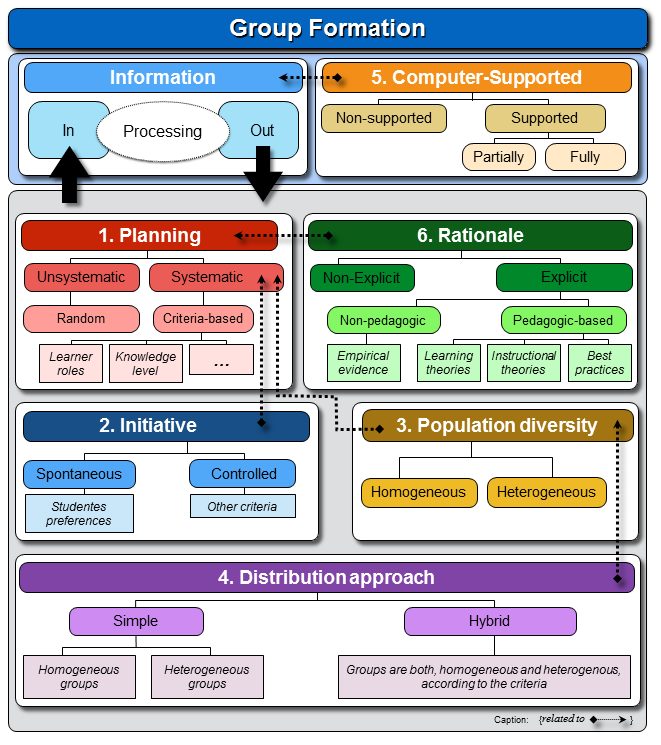
\includegraphics[]{gf_framework_full}
\end{figure}

Figure 1 gives an overview of our framework that can be used to classify, analyze and understand different types of research on the topic. The categories in the framework are tailored to give an overview of the efforts that have been carried out in the area, support the comprehension of the most investigated topics, and highlight the interacting and overlapping topics. Nevertheless, it is worth emphasizing the categories we came up with are not exhaustive. That is, they do not cover all the dimensions of the research spectrum of group formation in the context of CSCL. For example, the group activities were planned to occur face-to-face or in a distance learning way? The activities will occur synchronously or asynchronously?

In addition, we created three categories not showed in Figure 1. The purpose of these categories is to support gathering information about the way the selected researches have being conducted, and not directly about the group formation process.

\begin{itemize}
\item Educational level (or learning activities): By analyzing in which in educational contexts group formation has been explored, one can determine research gaps and future research opportunities;
\item Research methods: This category characterizes the type of research that has been carried out and reported in the studies;
\item Publication type: As for the publication types, we have selected primary studies that have been published in conferences, journals, and workshops.
\end{itemize}

%------------------------------------------------------
% Study 2
%------------------------------------------------------
\section{Study 2: Towards a Conceptual Framework for Bridging Player and Learner Roles}

Gamification is highly context-dependent, and ill-designed gamification solutions can lead to harmful effects instead of the expected benefits [4, 5]. Thus, the construction of sound gamified CL sessions requires not only careful analysis of appropriate gamified activities (e.g., environment’s design) and meaningful rewards (e.g., suitable game elements) but also, the ability of assigning appropriate player roles to each learner. Towards filling such a gap, we set out to create a conceptual framework to handle models and vocabulary to represent learner-player roles interactions. 

In Chapter \ref{chapter:background-cscl} we briefly introduced some CSCL concepts , such as group formation and in

and in Chapter \ref{chapter:persuasive-techonology}, we presented  

This chapter will use these concepts and will show the models we devised as well as the vocabulary gathered and organized to represent learner-player roles interactions in gamified CL contexts.

Our approach for creating player roles is based on the Motivations to Play  proposed by [19]. In [19], differently from most available player models, instead of using psychological archetypes in an effort to fit a player in one kind of dominant personality type, the proposed approach tries to identify not only the reasons that can motivate an individual to play a video game,  but also their relationship and overlaps. In this way, the model proposed by [19] does not attempt to identify in which archetype one individual fits, but rather to understand what can motivate such an individual to play. In addition, by identifying the reasons that may arouse motivation to play, by analyzing the results of the scoring system developed, one can also identify what can be deemed less attractive for such an individual. 
To help us better understand player’s needs that drive motivations to play, we rely on Self-determination Theory (SDT) concepts [13]. SDT seeks to explain how intrinsic and extrinsic motivators influence human behavior and the development of individuals. The three basic psychological needs, considered fundamental to influence motivation are autonomy, relatedness, and competence. According to [13], by promoting the internalization of these feelings, individuals have the potential to carry out their activities with improved performance, persistence, and creativity, for instance. 

\begin{table}[]
\centering
\caption{Motivations to play (Yee, 2008) X STD (Ryan and Deci, 2001) X Player role (also Ferro et al., 2013)
}
\label{my-label}
\begin{tabular}{|l|l|c|c|c|l|}
\hline
\multicolumn{2}{|c|}{\textbf{Motivations to play}} & \multicolumn{3}{c|}{\textbf{Self-Determination Theory}} & \multicolumn{1}{c|}{\textbf{Player role}} \\ \hline
Component & Subcomponent & \multicolumn{1}{l|}{Competence} & \multicolumn{1}{l|}{Relatedness} & \multicolumn{1}{l|}{Autonomy} &  \\ \hline
\multirow{3}{*}{Achievement} & Advancement & x &  &  & \multirow{2}{*}{Achiever} \\ \cline{2-5}
 & Mechanics & x &  &  &  \\ \cline{2-6} 
 & Competition & x &  &  & Conqueror \\ \hline
\multirow{3}{*}{Social} & Socializing &  & x &  & \multirow{3}{*}{Humanist} \\ \cline{2-5}
 & Relationship &  & x &  &  \\ \cline{2-5}
 & Teamwork &  & x &  &  \\ \hline
\multirow{4}{*}{Immersion} & Discovery &  &  & x & Explorer \\ \cline{2-6} 
 & Customization &  &  & x & Creator \\ \cline{2-6} 
 & \textit{Role-playing}* &  &  &  &  \\ \cline{2-6} 
 & \textit{Escapism}* &  &  &  &  \\ \hline
\end{tabular}
\end{table}


\begin{table}[!htb]
\centering
\caption{Player roles description}
\label{my-label}
\begin{tabular}{|l|l|l|}
\hline
\textbf{Player role} & \textbf{Description} & \textbf{Source} \\ \hline
\begin{tabular}[c]{@{}l@{}}Achiever\\   (goal-oriented)\end{tabular} & \begin{tabular}[c]{@{}l@{}}They enjoy not only completing a game,
but also being the best winner, accumulating\\
all rewards the game can offer. They are motivated by\\
receiving glory (points, titles, medals, trophies,\\
achievements); gathering (virtual currency and\\
goods); and collecting rare or all in-game items\\
(equipment, weapons, armor, vehicles, mounts, pets).\end{tabular} & {[}19, 24, 26–28{]} \\ \hline
\begin{tabular}[c]{@{}l@{}}Conqueror\\   (people-oriented)\end{tabular} & \begin{tabular}[c]{@{}l@{}}They enjoy rushing and competing against other people.\\ 
Usually, they enjoy testing their skills and seeing\\
how they stack up against other people. They find\\
external ranking systems and zero-sum game mechanics\\
appealing.\end{tabular} & {[}19, 24, 27, 28{]} \\ \hline
\begin{tabular}[c]{@{}l@{}}Humanist\\   (people-oriented)\end{tabular} & \begin{tabular}[c]{@{}l@{}}They enjoy socializing with people (e.g.,\\
being part of groups and teams, forming\\ 
partnerships, and playing collaborative games).\\
They value socializing, sharing learning, and\\
relationship building via shared tasks.\end{tabular} & {[}19, 24, 27, 28{]} \\ \hline
\begin{tabular}[c]{@{}l@{}}Explorer\\   (system-oriented)\end{tabular} & \begin{tabular}[c]{@{}l@{}}They enjoy exploring the system by\\
discovering the ins-and-outs (e.g., hidden or\\
remote places, finding loopholes, knowing the\\
rules that govern a space).\end{tabular} & {[}19, 24, 27, 28{]} \\ \hline
\begin{tabular}[c]{@{}l@{}}Creator\\   (system-oriented)\end{tabular} & \begin{tabular}[c]{@{}l@{}}They enjoy customizing the system (e.g.,\\ 
backgrounds, fonts, buildings, characters,\\
armor, weapons, and vehicles).\end{tabular} & {[}19, 24, 26–28{]} \\ \hline
\end{tabular}
\end{table}

%------------------------------------------------------
% Study 3
%------------------------------------------------------
\section{Study 3: Brazilian Portuguese Cross-Cultural Adaptation and Validation of the Sensibility to Persuasion Scale (Br-STPS)}

%------------------------------------------------------
% Study 4
%------------------------------------------------------
\section{Study 4: Persuasion Profiling to Cope with Learners' Willingness to Join Groups in CSCL}

%-------------------------------------------------------
% Concluding Remarks
%-------------------------------------------------------
\section{Concluding Remarks}

\chapter{Results}
\label{chapter:results}
%------------------------------------------------------
% Study 1
%------------------------------------------------------
\section[Study 1]{Study 1: Framework to Understand and Classify Research in CSCL}

%------------------------------------------------------
% Study 2
%------------------------------------------------------
\section[Study 2]{Study 2: Towards a Conceptual Framework for Bridging Player and Learner Roles in Gamified Collaborative Learning Contexts}

%------------------------------------------------------
% Study 3
%------------------------------------------------------
\section[Study 3]{Study 3: Brazilian Portuguese Cross-Cultural Adaptation and Validation of the Sensibility to Persuasion Scale (Br-STPS)}

%------------------------------------------------------
% Study 4
%------------------------------------------------------
\section[Study 4]{Study 4: Learners' Willingness to Join Constraint-based CSCL Groups}

%------------------------------------------------------
% Study 5
%------------------------------------------------------
\section[Study 5]{Study 5: Persuasion Profiling to Cope with Learners' Willingness to Join Groups in Gamified CSCL Environments}


%------------------------------------------------------
% Summary
%------------------------------------------------------
\section{Summary of the results}

\chapter{Discussions}
\label{chapter:discussions}
% This chapter revisits the research problem and the RQs (Section 7.1). Drawing on the
% findings of our investigation, we further elaborate on the advantages and disadvantages
% of extending JIT compilers to support software testing techniques (Section 7.2). This
% chapter also restates the contributions (Section 7.3), discusses the current limitations
% (Section 7.4) of our proof-of-concept implementation, and suggests future research directions
% (Section 7.5). The chapter concludes with a discussion of the relevance of this research and
% a summary of the technical challenges faced when extending Maxine VM (Section 7.6).

\section{Contributions}

\section{Theoretical implications}

\section{Practical implications}

\section{Limitations}

\section{Future work}

\section{Overall Conclusions}



% ---
% Finaliza a parte no bookmark do PDF, para que se inicie o bookmark na raiz
% ---
\bookmarksetup{startatroot}% 
% ---

% ----------------------------------------------------------
% ELEMENTOS PÓS-TEXTUAIS
% ----------------------------------------------------------
\postextual

% ----------------------------------------------------------
% Referências bibliográficas
% ----------------------------------------------------------
\bibliography{references}

% ---------------------------------------------------------------------
% GLOSSÁRIO
% ---------------------------------------------------------------------

% Arquivo que contém as definições que vão aparecer no glossário

% \newword{HTTP}{Hypertext Transfer Protocol is an application protocol for distributed, collaborative, and hypermedia information systems. HTTP is the foundation of data communication for the World Wide Web.}

\newglossaryentry{Latex}
{
    name=Latex,
    description={Is a mark up language specially suited 
    for scientific documents}
}

\newglossaryentry{Nintendo}
{
    name=Nintendo,
    description={Japanese multinational company headquartered in Kyoto, Japan}
}

\newglossaryentry{Systematic mapping}
{
    name=Systematic mapping,
    description={a method that involves searching the literature for gauging the extension and the amount of primary studies}
}

\newglossaryentry{Primary studies}
{
    name=Primary studies,
    description={published articles in a given field of interest}
}

% Comando para incluir todas as definições do arquivo glossario.tex
\glsaddall
% Impressão do glossário
\printglossaries

% ----------------------------------------------------------
% Apêndices
% ----------------------------------------------------------

% ---
% Inicia os apêndices
% ---
\begin{apendicesenv}

    \chapter{Group Formation in CSCL Environments: Systematic Mapping}
    \label{chapter:gf_mapping}
    %---------------------------------------------
% The Systematic Mapping Process
%---------------------------------------------
\section{The Systematic Mapping Process}

As a research area advances, the amount of studies published in that area tends to increase. Thus, obtaining an overview of an established research area can be a complex undertaking. Evidence-based Software Engineering (Dybå et al. 2005) proposes a set of guidelines to support the conduction this sort of investigation. More specifically, these guidelines outline how to identify, evaluate, interpret, and analyze primary studies (Dybå and Dingsøyr 2008). The main assumption is that those guidelines, which are expressed and embodied in systematic mappings and systematic reviews, lead to more consistent results that can be more easily replicated.
Therefore, to obtain a bird's eye view of the approaches that have been used for group formation within CL environments, we carried out a systematic mapping study. Systematic mappings are also known as scoping reviews (Pretorius and Budgen 2008), and they involve methodologically searching the literature to ascertain the nature and broadness (i.e., type and amount of primary studies) of the existing, published research on a particular topic (Magnisalis et al. 2011). In research, primary studies are examples of original research (Kitchenham 2004)

The systematic mapping herein described is based on the guidelines proposed by (Petersen et al. 2008) According to (Petersen et al. 2008), the key steps of a systematic mapping are the following: (i) definition of research questions (RQs), (ii) searching for relevant studies, (iii) screening of studies, (iv) keywording of abstracts, and (v) data extraction and mapping. Figure 1 illustrates these steps as well as the order in which they are performed. As shown in Figure 1, the conduction of each step results in an intermediate result. The main contribution of a systematic mapping is made up of these intermediate results. The following subsections briefly describe how we carried out the steps in Figure 1 and the intermediate outcomes of these steps.

\textbf{Figure 1. Systematic mapping main steps (Petersen et al., 2008).}

%---------------------------------------------
% Definition of the Research Questions
%---------------------------------------------
\subsection{Definition of the Research Questions}
 
As mentioned, the main goal of this systematic mapping is to gather data on and look at the state-of-the-art of research on group formation in the context of CSCL environments. It is worth mentioning that the RQs in a systematic mapping are framed in such a way as to drive the selection of primary studies and the analysis that takes place in the subsequent steps. The RQs that drove this systematic mapping are outlined in Table 1.

\textbf{Table 1. Research questions on the study.}

During this step we also defined the scope of our systematic mapping, outlining its population, intervention and expected results: 
Population: primary studies examining varying aspects of the formation of groups in the context of CSCL.
Intervention: primary studies that either apply, discuss, or propose strategies, approaches methods, or techniques for group formation or report on experiences with group formation.
Expected Results: an overview of the state-of-the-art of group formation. It is expected that, apart from providing a summary of what has been investigated in this research area, the results contribute to the identification of new avenues for research on group formation applied to CSCL by highlighting areas require more research.

%---------------------------------------------
% Searching for Relevant Studies
%---------------------------------------------
\subsection{Searching for Relevant Studies}

We created a search string by combining some terms, their synonyms, and acronyms. The initial set of terms was defined after an interview with a specialist and based on the preliminary scanning of 10 primary studies manually selected. The final set of terms is shown in Table 2. The search encompassed the electronic databases that are deemed as the most prominent scientific sources and, therefore, prone to include relevant primary studies (Dybå et al. 2007). We searched the following electronic databases: ACM Digital Library, IEEE Xplore, Elsevier (via ScienceDirect), Springer (via ScienceDirect), Wiley Online Library, Web of Science, EngineeringVillage and SCOPUS. It is worth mentioning that we did not place any restrictions on date of publication when searching for primary studies. 

\textbf{Table 2. Terms used in electronic libraries for the research of systematic mapping}

Table 3 presents the total amount of papers returned, the number of candidate studies after skimming through titles and abstracts, and the final set of primary studies. The next subsection elaborates on how we arrived at the final set of primary studies.

\textbf{Table 3. Total of returned papers, selected candidates, and the final set.}

%---------------------------------------------
% Screening
%---------------------------------------------
\subsection{Screening}

The purpose of this step is to assess the suitability of primary studies with respect to the RQs. Therefore, in this step; all papers are evaluated against predefined inclusion and exclusion criteria that reflect the RQs. After applying these criteria (Table 4) to titles and abstracts, the initial set containing 3571 papers was reduced to 423 candidate studies. After going over the candidate set, we ended up with 106 primary studies (Figure 2).

Figure 2. Overview of the systematic searching process.

Table 4. Inclusion and exclusion criteria for screening of returned items.

Figure 3 shows the frequency of research on group formation in the context of CSCL over time. As can be seen in Figure 3, the formation of groups has been investigated for approximately 20 years. Moreover, the amount of papers on this topic has dramatically increased since 2006. In particular, 2009 and 2011 stand out as the years in which most efforts in this area have been published so far: 16 studies in 2009 and 17 in 2011. 

Figure 3. Frequency of selected primary studies distributed by year of publication.

%---------------------------------------------
% Keywording
%---------------------------------------------
\subsection{Keywording}

This step is centered on classifying and categorizing primary studies. Initially, the abstracts of the primary studies were scanned for keywords that reflect the contributions presented in these studies. Thereafter, the resulting keywords were merged (i.e., terms that were considered synonyms were collapsed into the most commonly occurring term between the two) and analyzed in hopes of gauging the nature of the contributions in this area. 
We use the keywording to classify the studies according to our framework and answer the RQs that we set out to investigate. Note that primary studies can fall into more than one category in our framework; thereby some of the proposed categories overlap.

%---------------------------------------------
% Systematic Mapping Results
%---------------------------------------------
\section{Systematic Mapping Results}

In this section, we analyze the results of our systematic mapping. We draw information from the primary studies in order to answer the RQs of our mapping study. 

%---------------------------------------------
% \subsection{Research Question 1: What are the most investigated characteristics of group formation in the domain of CSCL?}
%---------------------------------------------
\subsection{Research Question 1: What are the most investigated characteristics of group formation in the domain of CSCL?}

The categories, as mentioned earlier, were created with the purpose of shedding some light on what are the most investigated characteristics of group formation in the domain of CSCL. By characteristics we mean that we applied a keywording strategy to prepare our rating system and characteristics for the selected primary studies. By applying such a strategy, initially summaries were read to find keywords and concepts that reflect the study's contribution. Next, these keywords and concepts were combined to produce a general understanding of the nature and contributions of the research. The classification scheme gradually evolved towards its final version as some characteristics were eliminated, added, merged or split (Durelli et al. 2010).
Also, by grouping the primary studies into categories allowed us better to grasp the interrelationships among categories and how efforts in this area overlap. However, it is worth mentioning that the resulting categories do not encompass all characteristics, research themes and contributions in the area. Rather, the categories were devised in hopes of better answering the RQ1.

%---------------------------------------------
% \subsubsection{Group Formation Planning}
%---------------------------------------------
\subsubsection{Group Formation Planning}

As mentioned, this category groups the primary studies in terms of the sort of planning that was used during group formation. Here we classify as unsystematic group formation approaches within which the formation of groups lacks a set of governing rules and takes places in a seemingly random fashion. In contrast to unsystematic group formation, systematic group formation is based on criteria that govern the size and organization of groups. Figure 5 shows the proposed classification, highlighting the basic difference between systematic and unsystematic group formation. In 12 of the selected studies, students are grouped in a random fashion. Nevertheless, in only 6 of these studies randomness is the only factor determining group formation. In the other studies, it was also possible to group students based on criteria aimed at achieving the target educational objectives. As an example, in the study conducted by (Mujkanovic and Lowe 2012), initially the groups were unsystematic formed (i.e. by chance), given that not enough information to warrant the application of more complex criteria about the students was collected yet. Later, after the conduction of more activities, the students were evaluated, and the results of the evaluations were then used as a group formation criterion. According to (Mujkanovic and Lowe 2012), this approach could be an alternative to using placement or pre-evaluation questionnaires. One drawback of using questionnaires before collaborative learning activities is that carrying out this sort of evaluation takes a significant amount of time, and it is often seen as tedious for the students taking part in it. 

Figure 5. Classification scheme of the primary studies in accordance with in terms of the sort of planning that was used during group formation.

Most primary studies, however, report on group formation approaches that are based on some criteria: in 94 studies, criteria are used to support the definition of rules that establish which group each student should be added to. Figure 6 shows the frequency of the criteria for the formation of groups found in primary studies analyzed. The number of criteria present in each study varies according to the objectives of the collaborative activities to be performed or can be based on the kind of computational support employed (e.g. algorithms). Abnar et al. (2012) remark that, in general, when groups are manually created, only one criterion is used. They also point out that the more criteria are used, the more complicated it is to handle the information related to groups. Nevertheless,  Medina and Gómez-Pérez (2013), and Hwang et al. (2008) state that it is unlikely coming up with one criterion that yields good groups. It follows that it is desirable to have multiple criteria, given; the more information is taken into account during group formation, the greater the control over the quality and granularity of the resulting groups. Recent research indicates that sound pedagogical theories should underpin group formation approaches. For instance, the studies carried out in Isotani et al. (2009) and Isotani et al. (2013) provide further evidence in this regard. Moreover, the approaches proposed in Isotani et al. (2009) and Isotani et al. (2013) benefit from Semantic Web to formalize the knowledge required for creating groups. 
	The most used criterion for group formation was knowledge level. Knowledge level-based group formation is investigated in 59 primary studies. Skill-based group formation is the second most investigated criterion, investigated in 33 primary studies. Learner roles are the third most investigated criteria, 31 primary studies. As shown in Figure 6, the other criteria that have been explored are group objectives, individual objectives, students genre, cultural aspects (e.g., nationality and language), interaction issues, characteristics extracted from social relationships, psychological characteristics, learning disabilities, schedule compatibility, age, and academic formation. It is worth mentioning that these are only some of the identified criteria, studies might have used other additional criteria. However, these other criteria were not mapped because the studies failed to describe sufficiently them. Usually, these additional criteria are simply mentioned in the primary studies as “other criteria” or “among other things”.

Figure 6. Frequency of the criteria for the formation of groups found in primary studies analyzed.

%---------------------------------------------
% \subsubsection{Initiative in Systematic Group Formation}
%---------------------------------------------
\subsubsection{Initiative in Systematic Group Formation}

When group formation follows a methodical (viz., systematic) approach to group formation, the initiative for group formation can be handled in two different ways: spontaneous group formation (i.e., when the students are the ones in charge, yielding self-selected groups) and controlled group formation (i.e., when the instructor or underlying approach controls group formation, resulting in instructor-select groups). This distinction is highlighted in Figure 7. We classify as spontaneous the approaches in which students are free to form their own groups. Spontaneous group formation approaches take into account the preferences of the students (e.g., affinity between students, idiosyncrasies, and friendship). Therefore, we classified as controlled group formation (guided) the approaches that take some other elements into account during the formation of groups, apart from students’ preferences. We argue that the term controlled better describe such approaches, given that there is an external element, which can be impervious to the students’ preferences, effectuating the rules and controlling how students should be grouped.
 
Figure 7. Classification of primary studies in accordance with the initiative of group formation.

In 21 of the selected studies, the preference of the studies was taken into account during group formation. Nevertheless, in only four studies this was the only factor taken into consideration. In the other 17 studies, apart from the students’ preferences, other criteria could also be used. In these primary studies, the students are polled about their preferences, and the gathered information is then used to devise group formation criteria.
The Venn diagram shown in Figure 8 illustrates how the primary studies were categorized in terms of their planning strategy. As mentioned, some primary studies can fall in more than one category since their approaches are flexible enough to allow for more than one planning strategy. By analyzing Figure 8, it can be seen that most group formation approaches (70 primary studies) are exclusively criteria-based approaches.

Figure 8. Distribution of the primary studies according to the criteria used during the clustering strategy.

%---------------------------------------------
% \subsubsection{Population Diversity}
%---------------------------------------------
\subsubsection{Population Diversity}

In the context of this study, diversity has to do with the makeup of groups, which can be heterogeneous or homogeneous as shown in Figure 9. Homogeneous approaches emphasize criteria that result in groups of like-minded students, i.e., students that present similar characteristics. Heterogeneous approaches, conversely, propose the creation of groups that are comprised of members with different backgrounds and characteristics. 

Figure 9. Classification scheme for the audience diversity when forming groups.

The most used approach is the formation of heterogeneous groups (84 primary studies). Evidence suggests that heterogeneous groups foster the interaction among group members due to the members have skills that are complementary to the group as a whole (Barkley et al. 2005; Johnson and Johnson 1999). Also, in heterogeneous groups it is normal to have members with characteristics that supplement other individuals in the group. 
In 36 primary studies relied on the formation of homogeneous groups. Note that in two of these 36 studies the formation of homogeneous groups is the only option, the other 34 studies also propose criteria that yield heterogeneous groups (Figure 10). Also, nine papers were not classified in terms of diversity, given that in five of them the formation of groups can be carried out in a random fashion and four in a spontaneous way. Apart from these papers, we also analyzed 17 primary studies that either use or investigate group formation. However, it was not possible to identify the diversity of the groups in these papers.

Figure 10. Primary studies according to diversity of the population in the groups.

In the study conducted by Chiu and Hsiao (2010), it is argued that randomly assembled groups can result in an acceptable level of heterogeneity with respect to certain characteristics as, for instance, the amount of students of the same gender or with some particular personality traits (e.g., active students, passive students, leaders, and followers). Moreover, in the study conducted by Ardaiz-Villanueva et al. (2011), problem-based learning (PBL) principles and several support tools were used to support the conduction of collaborative learning activities. Two criteria drive group formation: the first is based on a “creativity score” attributed to each student and the second boils down to computing an “affinity score” that gauges how each student gets along with others. According to the authors, the results seem to suggest that homogeneous group (in terms of creativity) and whose members interact with each other well lead to a better learning experience. Besides, the authors report that in this kind of groups they did not detect freeloaders and there was an increase in students’ engagement during collaborative learning activities.

%---------------------------------------------
% \subsubsection{Distribution Approaches}
%---------------------------------------------
\subsubsection{Distribution Approaches}

We categorized the studies according to the way the students were distributed in groups. As mentioned, groups can be homogeneous or heterogeneous groups according to the criterion (or criteria) used. In terms of distribution, we classified the studies whose approaches result in either homogeneous or heterogeneous groups (despite how many criteria were used) as simple distribution. By the other hand, we also found studies in which a subset of criteria was used to cluster the students in homogeneous groups, while at the same time; another subset of criteria was used to cluster them in heterogeneous groups. This second type of approach was classified as hybrid distribution, and the classification scheme is shown in Figure 11.

Figure 11. Simple distribution results in homogeneous OR heterogeneous groups, while in hybrid distribution, groups are concomitantly homogeneous AND heterogeneous according to each subset of criteria.

%---------------------------------------------
% \subsubsection{Computational support}
%---------------------------------------------
\subsubsection{Computational support}

Although the domain of computer-supported collaborative learning contains the words "computer-supported", not always the group formation occurs with technological support. Based on these observations, we devise the category shown in Figure 12, to classify the primary studies according the computational support. 

Figure 12. Classification of the primary studies according to the computational support.

We observed that a few primary studies (13) did not provide enough information clarifying neither the use nor the extension of the computational support, getting this restricted to the other stages of collaborative learning (i.e. collaborative tasks to be performed). In the remaining 83 studies analyzed, various technological solutions have been used. Although the extent and the way these technologies were employed are relevant, they are beyond the scope of this paper and will not be detailed. Table 5 presents an overview of the related major computational resources identified in the studies analyzed, and Table 6 presents the main types of algorithms described in the primary studies. 

Table 6. Major algorithms used to support group formation in the primary studies investigated.

%---------------------------------------------
% \subsubsection{Rationale Behind the Strategy for Group Formation}
%---------------------------------------------
\subsubsection{Rationale Behind the Strategy for Group Formation}

The primary studies were also classified in terms of how the authors back up their approach for group formation. We found three types of studies: (i) studies that do not present any arguments that back up their approaches, (ii) studies whose group formation approach is borne out by empirical evidence, (iii) and studies that draw on assumptions from pedagogical theories (Figure 13). 
 
Figure 13. Classification of the primary studies regard the kind of rationale found in the primary studies explaining the group formation approach.

Only 37 of the 106 analyzed studies are based on sound pedagogical or instructional theories, which back up the selection criteria employed during group formation. We also found that 46 studies do not report whether any pedagogical theory was used to support the group formation criteria. These 46 studies mention, however, that the chosen criteria are based on empirical evidence. Apart from these primary studies, 23 studies do not elaborate on what theories ground their criteria. Table 7 shows an overview of the rationales behind the examined group formation approaches.

Table 7. Regard the kind of rationale found in the primary studies explaining the group formation approach.


%---------------------------------------------
% \subsubsection{The answer for RQ1}
%---------------------------------------------
\subsubsection{The answer for RQ1}

RQ1: What are the most investigated characteristics of group formation in the domain of CSCL?

A\textsubscript{RQ1}:: The majority of the primary studies (101 out of 106) report on approaches for planned group formation, i.e., the formation of groups is based on pre-established criteria. The most widely used criterion is the level of knowledge of the students, which is used in 46 of the selected studies. Controlled group formation is used in 90 primary studies. In terms of distribution, most primary studies rely on heterogeneous groups: 84 studies propose the formation of heterogeneous groups. Nevertheless, only in 50 out of these 84 studies simple heterogeneous groups are the only possible outcome. According to our results, 82 studies capitalize on some sort of technology to automate and support group formation. Only 37 studies exploit educational or pedagogical theories to justify their rationale for the group formation approach. 

%---------------------------------------------
%\subsection{Research Question 2: In what educational level (or learning activities) group formation has been most investigated and applied to?}
%---------------------------------------------
\subsection{Research Question 2: In what educational level (or learning activities) group formation has been most investigated and applied to?}

In order to answer RQ2, we classified the selected studies in terms of their target population. In the context of this paper, target population refers to the stage (or level) at which educational activities take place or the type of educational activities. As shown in Figure 14, the group formation approaches proposed in most studies (56) emphasize tertiary education (viz., undergrad students). Few studies focus on applying group formation approaches to other educational levels (or stages). For instance, our results would seem to suggest that there has been scant research on the impact of group formation when applied to early childhood education (1), graduate students (1), e-Health students (1), language-learning activities (1), primary education students (3), and secondary education students (6). 36 primary studies fail to specify the target population of their proposed approach. Also, these studies present theoretical models that represent solutions that have not been implemented or fully tested yet.
 
Figure 14. Distribution of primary studies according to the level/type of educational activity.

%---------------------------------------------
% \subsubsection{The answer for RQ2}
%---------------------------------------------
\subsubsection{The answer for RQ2}

RQ2: In what educational level (or learning activities) group formation has been most investigated and applied to?

A\textsubscript{RQ2}:: Most research on group formation applied to CSCL has been geared towards undergrad students: approximately 52\% (56 primary studies) of the studies tackle group formation at this educational stage (level). 

%---------------------------------------------
%\subsection{Research Question 3: In what educational level (or learning activities) group formation has been most investigated and applied to?}
%---------------------------------------------
\subsection{Research Question 3: What type of research is the most common in the field?}

Our answer is based on the classification proposed in (Wieringa et al. 2005), which comprises the following research types. Validation Research, studies that fall into this category describe a novel technique, approach, or strategy and have not been implemented in practice, but its effectiveness has been evaluated to some degree through laboratory studies. Evaluation Research, this category contains studies that empirically evaluate a technique, approach, or strategy in practice or real settings. Position Papers, these studies report the authors' point of view. Research in this category does not contain evidence that backs up the authors' opinion. Philosophical Papers, studies that present a new of perceiving things or new guidance for a domain, often using taxonomies and conceptual frameworks. Solution Proposals, Studies in this category are usually not present in-depth validation of the described technical solution but tend to describe a proof of concept by way of example or a sound prototype running. Experience papers, these studies are concerned with reporting the author's experience during the implantation of a new approach. As some selected primary studies did not fit well into the categories above, we extended the classification scheme, by adding a research type category namely Tools. In this category are the studies whose main contribution is the developed tool, often in the form of a research prototype. 

After reading the primary studies, we identified four research methods. As indicated in Table 8, the research methods in the primary studies fall into one of the following categories: (i) Solution proposals, (ii) Evaluation, (iii) Opinion, and (iv) Tools. Solution proposals are by far the most common research method, including 77 studies, 17 primary studies are concerned with some evaluation, and only one study falls into the opinion category. Moreover, the main contribution presented by 11 studies boils down to the implementation of a tool to automate and support group formation, falling into the tools category.

Table 8. Distribution of primary studies by research type.

%---------------------------------------------
% \subsubsection{The answer for RQ3}
%---------------------------------------------
\subsubsection{The answer for RQ3}

RQ2: What type of research is the most common in the field?

A\textsubscript{RQ3}:: The research method used in the majority of the primary papers is solution proposal: 77 studies present group formation approaches that can be applied to CSCL environments. Conversely, the least explored category is opinion. Only one study describes the author’s view about group formation applied to CSCL environments and the implications thereof\todo{verificar este final!}.

%---------------------------------------------
%\subsection{Research Question 4: What are the main venues in which research in this area has been published?}
%---------------------------------------------
\subsection{Research Question 4: What are the main venues in which research in this area has been published?}

As shown in Figure 15, most primary studies are indexed in IEEE (IEEE Xplore) and Elsevier (26 and 24 papers, respectively). ACM Digital Library indexes 19 of the selected papers, 14 papers were retrieved from Scopus, and Springer and Web of Knowledge (WoK) had six papers each. The electronic database with the least amount of selected papers was Engineering Village (5 papers). It is worth mentioning that Springer, WoK, and Engineering Village were the last electronic databases we went through; consequently many of the papers returned by these sources had already been retrieved and selected from other databases. Apart from these studies, 6 selected journal papers were retrieved from SciVerse Hub. 

Figure 15. Frequency of selected primary studies according to the consulted electronic databases.

The selected papers were published in a variety of venues that range from conferences, workshops, to journals. Figure 16 shows an overview of the distribution of primary studies according to their types over the years. By analyzing Figure12, we can see that most efforts in the area were published from 2006 on. Since then, it seems that the topic has gained momentum. As indicated in Figure 16, there was a marked increase in the amount of journal publications in 2011. 

Figure 16. Frequency of selected studies according to the year and the publication of the forum.

As shown in Table 9, 12 venues has contributed with at least two studies that represent 48 publications, while the rest of the studies are spread in 58 different venues (with one publication each). 

Table 9. Main venues in which research about group formation has been published.

%---------------------------------------------
% \subsubsection{The answer for RQ4}
%---------------------------------------------
\subsubsection{The answer for RQ4}

RQ4: What are the main venues in which research in this area has been published?

A\textsubscript{RQ4}: Most primary studies were published in journals. Computers \& Education is the venue with the highest number of selected studies (10), followed by another journal, Computers in Human Behavior and for the proceedings of the Conference on Innovation and Technology in Computer Science Education (ITiCSE), both with six studies. 

%---------------------------------------------
% \section{Discussion}
%---------------------------------------------
\section{Discussion}

Drawing on the information from the primary studies, we identified that group formation usually encompasses three fundamental steps that resemble the input-process-output (IPO) model. In this context, group formation approaches receive information about students as input and then some processing or computation is performed on such information, and the outcome is information on how students should be placed in groups. Basically, these IPO steps can be performed (i) without a computational support (e.g. manually carried out by the instructor), (ii) be partially computerized (e.g. spreadsheets, LMS), or (iii) may be automatically carried out by a computer system.
Moreover, a central topic discussed in some of the primary studies is the strategy used to group students. As mentioned in Section 4, group formation can be carried out in a random fashion (i.e., by chance), or it can be controlled (i.e., criteria-driven group formation). As mentioned, criteria-driven group formation can fall into two categories: spontaneous group formation and controlled group formation. In the former, students are self-assigned to groups, yielding self-selected groups. In the latter, instructors or other agents handle group formation, resulting in instructor-formed groups. Evidence suggests that the main advantages of spontaneous group formation are related to self-motivation, which often leads to a more positive experience throughout the learning activities. However, since self-selected groups are made of participants that share common interests or get along with each other, the same self-selected groups might be repeatedly formed. A clear shortcoming of this approach is that some individuals might be left out. Thus, ostracized students might face difficulties coping with learning activities on their own, leading to unsatisfactory results. 
Clearly, the group formation strategy influences the diversity of groups. Random approaches tend to result in heterogeneous groups. Nevertheless, since groups are formed by chance, it is possible that this approach generates single-gender groups or groups whose most elements belong to a given gender. Another problem with random approaches is that they can also form groups of students that have already mastered the subject in question or groups whose students have struggled to grasp the subject. To enforce group member diversity, therefore making the students interacting with a broad range of peers, students can be clustered in groups based on some criteria. The use of criteria adds a much more fine-grained control over group formation. Moreover, using criteria, it is also possible to create hybrid groups. As mentioned, hybrid group formation approaches employ a multitude of criteria to place students in groups that can be homogeneous and heterogeneous at the same time. However, when more criteria are employed; more information needs to be processed: this means that as the number of criteria increases, the need for computational support also becomes more critical. In our systematic mapping, we found that hybrid group formation is proposed along with tools that automate group formation. 
Devising effective and theoretically sound group formation approaches is a notoriously complex task. Group formation approaches have to take into account many factors as for instance: (i) students’ knowledge, (ii) how students interact with each other, (iii) preferences, needs or limitations of the instructors, environment and students. Given the importance of well-founded group formation approaches, we set out to investigate the rationale behind the approaches proposed in the primary studies. In a way, all primary studies justify the usefulness of their approaches. Some studies, however, fail to describe the theories, concepts, and ideas that underpin their group formation approach. This can be a worrisome finding since, according to the impossibility of justifying either theoretically or pedagogically the selection of participants to compose a group is one of the main weaknesses of the available methods, and a strong reason for teachers’ hesitation in adopting systems with group formation capabilities.
Finally, in order to clarify the classification scheme elaborated; we analyzed the group formation approach proposed by, as follows. In Figure 17, the results of the analysis using such classification scheme are synthesized.

\begin{enumerate}
\item Planning - The paper aims in proposing a systematic criteria-based method for group formation that relies on genetic algorithms to process three characteristics of the students: student knowledge levels, student communicative skills, and an estimate of student leadership skills.
\item Initiative - The system is in charge of clustering the students based on the chosen criteria. 
\item Population diversity – The criteria are used to form both, homogeneous and heterogeneous groups.
\item Distribution approach – A hybrid approach is used since, the authors main goal is to achieve groups that are as similar as possible (homogeneous) to some characteristics of the total sample of students, however also taking into account the heterogeneity of each one. 
\item Computer-supported – Genetic algorithms are used to optimize the odds of using an arbitrary number of student characteristics to form hybrid groups.
\item Rationale – The group formations approach was tested with undergrad students; however, we were not able to identify the justification (neither pedagogic nor instructional) regards the selection of the audience, the learning process, and the learning goals. Still, the study justifies the group formation approach backing up on the benefits of using genetic algorithms to manipulate and manage a considerable amount of students’ characteristics. The paper comments that these three characteristics were based on a literature review.
\end{enumerate}

Figure 17. This figure shows the characterization of the research conducted by Moreno et al. (2012), the characterization follows the classification scheme created in this systematic mapping presented in this section. 

%---------------------------------------------
% \section{Threats to Validity}
%---------------------------------------------
\section{Threats to Validity}

A potential threat to validity is the inability to ensure that all relevant studies were selected. There is a possibility that some studies have been omitted considering that not all electronic databases were consulted. However, all consulted electronic databases are considered important forums of publications, susceptible to contain relevant studies. Thus, it can be considered that the chances that relevant studies have been resolved, or at least been mitigated. Also, we cannot eliminate threats to the validity of the quality point of view of the selected studies, because, during the selection process, we have not assigned scores to the studies.
The research questions and the inclusion and exclusion criteria were drawn up before performing the systematic mapping to ensure an impartial selection process. However, the consistency of the elaborate classification scheme can also pose a threat to validity since the knowledge to elaborate it is often only achieved at the end of the selection process (Dybå and Dingsøyr 2008).
It is important to mention that the difference between the initial quantity of articles and the final selection can be regarded as normal in this type of study. The main objective of a systematic mapping is to provide a broad overview of which have been published in the area of interest. Due this, one important characteristic of kind of study is to avoid imposing many restrictions on the selection of primary studies (Durelli et al. 2013).
Another possible threat to validity results from the operation of some electronic libraries and search systems. In some search engines, despite the use of keywords and wildcards, they often returned items fleeing the scope of the keywords used, therefore demanding further analysis of the undesired studies and manual intervention to eliminate them.

%---------------------------------------------
% \section{Concluding Remarks of the Systematic Mapping}
%---------------------------------------------
\section{Concluding Remarks of the Systematic Mapping}

This paper presented the results of our systematic mapping whose purpose was to provide an insightful overview of the current state of the art on group formation applied to CSCL. The categorization scheme we devised can be used to aid analyzing and understanding proposed group formation approaches. Moreover, it may be useful as a support tool to aid planning new ones. As a future work, we plan to optimize and extend the actual structure of the classification scheme. For example, as Massive Open Online Courses (MOOCs) are proliferating with huge number of participants with different backgrounds, culture and time zones (just to emphasize few points of interest) there is a need for new strategies for group formation in this kind of environment. Traditional approaches used for face-to-face learning or even in traditional e-Learning environments maybe can not be appropriate for MOOCs. Although 25\% of the studies state their approaches are suitable for online learning, only 1\% comment that their approaches are suitable for asynchronous group learning tasks, 7\% for synchronous, 19\% can be used in both scenarios, however, 74\% did not comment if the group interactions describe in the studies were planned to be executed synchronously or asynchronously.
Using the information extracted from the selected studies, we shed light on the most investigated approaches to group formation, the education stages in which these approaches are applied; the most used research methods, and the most common publication types. Besides the growing number of publications and the variety of computational approaches to support group formation, we identified that, the lack of presenting a rationale explaining the group formation approach can be a problem, and furthermore it can be exploited to open significant new opportunities for future research.
Group formation is one of the most important steps during the planning stages of CSCL activities. Due to the many elements that need to be taken into account during group formation, devising a sound group formation approach is considered a complex task. Although research in CSCL has come a long way, most group formation efforts fail to take into account motivational aspects during group formation. Rather, we found that most existing approaches emphasize the use of basic information about the students (e.g., proficiency) during group formation. 
Another contribution of our systematic mapping is that by analyzing its results it is possible to identify the ways in which group formation, when applied in the context of CSCL, has been explored so far. Thus, researchers can refer to this systematic mapping to determine research gaps and decide on future research directions. Finally, we conceive an infographic that summarizes all data presented in this paper, to provide a quick overview of the results presented (Available at: http://infografico.caed-lab.com/mapping/gfc/).











    \chapter{Gamification Applied to Education: Systematic Mapping}
    \label{chapter:gamification_mapping}
    In this study, we are focusing on providing an overview of the
research on gamification applied to education [5][16]. Furthermore,
it is worth mentioning that this mapping study is part of an ongoing
project whose purpose is to investigate gamification and Computer
Supported Collaborative Learning (CSCL). Thus, as a secondary
objective of this systematic mapping, we also aim to identify the
existence of initiatives that use gamification in CSCL
environments. 

\todo[inline]{FAZER O UPDATE E ESCREVER AQUI NOVOS  DADOS - CITAR O ONLINE QUANTO PRECISO}

%---------------------------------------------
% The Systematic Mapping Process
%---------------------------------------------
\section{The Systematic Mapping Process}

We carried out our study by following the process described by
[26]. According to them, systematic mappings are a fivefold
process: (i) definition of research questions, (ii) performing the
search for relevant primary studies, (iii) screening of papers, (iv)
keywording of abstracts, and (v) data extraction and mapping.
Research questions have to incorporate the study purpose. Thus,
since we set out to ascertain what aspect of gamification applied to
education has been most investigated by researchers, our three
research questions (RQs) reflect this purpose as the following:
RQ1: In what educational contexts and levels has gamification been
most investigated?
RQ2: What types of studies have been most investigated in
gamification and education?
RQ3: What gamification approaches have been most investigated
in the field of computer-supported collaborative learning (CSCL)?
Based on these questions we defined inclusion and exclusion
criteria. These criteria are important to identify relevant primary
studies that answer the RQs. We devised the following inclusion
criteria:
 If several papers reported the same study, only the most recent
paper was selected;
 If the paper describes more than one study, each study was
assessed individually.
And the following exclusion criteria:
 Papers that do not present studies relating to education;
 Papers in languages other than English;
 Technical reports and documents that are available in the form of
summaries or presentations (gray literature) and secondary
studies (i.e., systematic literature reviews and mapping studies).
At first, we ran some searches using a combination of candidate
keywords. These trial searches combined the keyword gamification
with some synonyms related to education and learning. Due to the
217
small number of papers returned from the resulting strings, we
decided that only the keyword gamification should be used.
This decision allowed us to analyze a greater number of papers,
lowering the odds of leaving relevant studies out of our final set.
Using gamification as keyword, we performed searches on
electronic databases that are known to cover relevant scientific
journals and articles from a wide variety of domains such as
Computer Science, Education and Educational Research, Science,
Engineering, Medicine and Psychology. Initially, we retrieved 357
primary papers. However, only 48 candidate papers were obtained
after applying the inclusion and exclusion criteria based upon title
and abstract. Finally, after going over introductions and
conclusions, we ended up with a final set of 26 primary papers as
shown in Table~\ref{tab:distribution_of_primary_studies}. The complete list of these papers can be obtained
at: http://goo.gl/KUH1m. 


\begin{table}[]
\centering
\caption{Distribution of primary studies by electronic database }
\label{tab:distribution_of_primary_studies}
\begin{tabular}{|l|l|}
\hline
\textbf{Database}         & \textbf{Quantity} \\ \hline
ACM Digital Library       & 144               \\ \hline
Elsevier (Science Direct) & 32                \\ \hline
IEEE Xplore               & 31                \\ \hline
Scopus                    & 95                \\ \hline
Springer                  & 55                \\ \hline
Total                     & 357               \\ \hline
Candidates                & 48                \\ \hline
Final Selection           & 26                \\ \hline
\end{tabular}
\end{table}

We read all 26 papers in full and applied a keywording strategy to
devise our classification scheme and categories for the selected
primary studies. At first, abstracts were read in order to find
keywords and concepts that reflect the contribution of the studies.
After reading the papers, the keywords and concepts were
combined to synthesize the nature of the selected contributions.
Finally, the final set of keywords was used to define representative
categories. As a result, the following categories were defined to
better understand and classify the primary studies:
Mastering Skills: in this category we included all studies that
propose the use of gamified systems as a means to improve
students' ability to perform activities considered complex or
repetitive.
Challenging: this category includes studies whose authors claim
that gamified systems that implement challenging activities can
contribute to the improvement of learning.
Guidelines: this category includes studies whose authors consider
how gamification can be applied in educational settings. These
studies, however, do not provide empirical evidence that backs up
the authors' claims. Usually, these papers are built on results of
other researchers.
Engagement: studies in this category describe approaches or
strategies to arouse and maintain students' interest in learning a
given subject.
Improving Learning: this category includes studies that propose
gamified solutions to enhance the way students learn, maximizing
the results of the learning process.
Behavioral change: this category includes studies that propose
using gamified systems in order to foster behavioral changes in
students.
Socialization: studies in this category discuss that learning can take
place under more favorable conditions when supported by gamified
social tools.

%---------------------------------------------
% Discussion - Analysis
%---------------------------------------------
\section{Discussion} 

In this section we analyze the results of our mapping study. The
purpose of this section is to give an overview of how gamification
has been used to support education. The information drawn from
the selected primary studies is also used to answer our mapping
study's research questions.
To answer our first question (i.e., in what educational contexts and
levels have gamification been most investigated?) we analyzed the
primary studies and categorized them according to the target
audience (Table~\ref{tab:target_audience}). In Table~\ref{tab:target_audience} we can observe that most primary
studies present gamification approaches tailored towards
supporting higher education students (46\%). Thus, we can conclude
that the answer to RQ1 is that gamification has been mostly applied
in approaches to teaching students in higher education. On the other
hand, among the selected primary studies, elementary education is
the stage of education drawing less attention: only two primary
studies, which accounts for only 8\% of the selected studies, discuss
gamification-based approaches for teaching elementary students.
As for the other studies, six primary studies (23\%) describe the
benefits and shortcomings of gamification-based models and
educational strategies. These six studies, however, fail to position
themselves in “the big picture”. In other words, the authors do not
mention in which educational level (e.g., elementary or higher
education) their approaches should be incorporated so that one can
best grasp the benefits of such approaches in particular educational
contexts. In fact, none of these six primary studies mention whether
or not gamification can be applied in educational level curricula.
 
\begin{table}[]
\centering
\caption{Primary studies categorized according to target
audience or subject matter}
\label{tab:target_audience}
\begin{tabular}{|l|r|r|}
\hline
\textbf{Target audience}   & \multicolumn{1}{l|}{\textbf{Number}} & \multicolumn{1}{l|}{\textbf{Frequency(\%)}} \\ \hline
Higher Education           & 12                                   & 46.15\%                                     \\ \hline
Non-specific context/level & 6                                    & 23.08\%                                     \\ \hline
Training and Tutorials     & 3                                    & 11.54\%                                     \\ \hline
Languages                  & 2                                    & 7.69\%                                      \\ \hline
Elementary Education       & 2                                    & 7.69\%                                      \\ \hline
Lifelong Education         & 1                                    & 3.85\%                                      \\ \hline
\end{tabular}
\end{table}

The other studies either discuss or propose using gamification
models with the following purposes: training and tutorials (12\%),
teaching and learning languages (8\%), and supporting students
tackling lifelong education \footnotetext{Further Education in Great Britain.}
 projects (1\%). It is worth mentioning that none of the selected studies described gamification approaches whose target audience is preschool, high school, or disabled
students.
There has been a recent growing interest in research on developing
e-learning environments that are equipped with gamification
elements and techniques. Table 3 presents the primary studies
clustered by date of publication. Although the first publications
appeared only in 2011, the number of studies on gamification more
than doubled from 2011 to 2012. As for 2013, taking into account
only January and February, the months during which this study was
carried out, three studies had already been published. It is important
to note that several articles related to gamification have been
published before 2011. Nevertheless, most of them were not related
to education and none of them met the inclusion/exclusion criteria
defined in our study. This result reveals that gamification applied
to education is becoming a new research trend with room for new
findings and improvements. To proper understand the impact
(positive or negative) and implications of using gamification in
educational contexts there is a need for more research and empirical
data. 

Table 3. Overview of the distribution of the selected studies
throughout the years

Most primary studies were published by either ACM DL (ACM
Digital Library) or Springer, as shown in Table 4. The electronic
databases, Elsevier (ScienceDirect) and IEEE (IEEE Xplore) had
five and three selected studies, respectively. We also searched
through Scopus, however, given that it was the last electronic
database to be examined, most primary studies it indexes had
already been selected from one of the aforementioned electronic
databases. Four studies were selected from Scopus; these studies
had not been returned by the other electronic databases. 

Table 4. Distribution of the primary studies according to
electronic database

By analyzing where the primary studies were published, we found
that there is no specific venue whose purpose is to bring together
research on gamification applied to education. The most notable
publication forums according to the number of selected primary
studies are the following: the American Society for Engineering
Education Annual Conference (ASEE) (two studies were published
in 2012) and the ACM eLearn Magazine (two studies as well).
Furthermore, three primary studies were book chapters from the
book Serious Games and Edutainment Applications published in
2011 by Springer [22].
Regarding the publication types, we have selected studies that have
been published in journals, magazines, conferences, workshops, symposia, and books. 

Table 5 gives an overview of the primary studies distributed according to publication type. As shown in Table 5, most selected studies are conference publications. Journal
publications are the second most common publication type. It is worth mentioning that most of these journals have a multidisciplinary scope. 

Table 5. Primary studies organized by publication type 

Primary studies frequently use the term “motivation” to justify the
research in question or the main reason behind investigating
gamification. Nevertheless, after an in-depth analysis of these
studies, we found that several objectives fall under the term
“motivation”. Thus, we were able to identify seven different
objectives: (i) Mastering skills: improving certain abilities of the
students; (ii) Challenging: proposing challenges that give extra
meaning to the learning process; (iii) Engagement: engaging
students in learning activities that are more interesting and easier to
follow; (iv) Improving learning: maximizing the acquisition of
knowledge; (v) Behavioral change: fostering changes of behavior
by rewarding adequate actions and penalizing unsatisfactory ones;
(vi) Socialization: allowing for both socialization mechanisms and
group learning; and (vii) Guidelines: discussing the benefits of
gamification as a means to motivate students and deal with some of
the learning process problems. Our results demonstrate that there
are some overlaps between these seven classification categories.
Apart from identifying the objectives of the primary studies, it is
also important to characterize the type of research that was carried
out and reported in these studies. Towards this end, we applied the
classification proposed in [26]. Such a classification comprises the
following research types.
Validation Research, studies that fall into this category describe a
novel technique, approach, or strategy that has not been
implemented in practice, but whose effectiveness has been
evaluated to some degree through laboratory studies.
Evaluation Research, this category contains studies that
empirically evaluate a technique, approach, or strategy in practice
or real settings.
Position Papers, these studies report the authors' point of view.
Research in this category does not contain evidence that backs up
the authors' opinion.
Philosophical Papers, studies in this category are similar to
position papers, however, they shed light on new ways through
which educational approaches can benefit from gamification.
Solution Proposals, studies that describe a solution technique,
approach, or strategy and argue for its usefulness, such a solution
is either novel or extends an existing approach; studies in this
category usually present examples and good line of argumentation
(but not strong empirical data). 
Experience papers, these studies are concerned with reporting the
author's experience during the implantation of a new approach.
Rather than plotting frequency tables to illustrate the distribution of
the studies according to research type and objectives, we decided
to generate a bubble plot (Figure 2), but the primary studies
summarized in Figure 2 are also shown in Table 6. The resulting
bubble plot is intended to be seen as a map of research on
gamification used in conjunction with education. A bubble plot has
two x-y scatter plots containing bubbles in category intersections.
The size of these bubbles is determined by the amount of primary
studies that have been classified in the pair of categories in
question.
Such a visual summary gives an overview that enables researchers
to pinpoint categories that have been drawing most attention as well
as the ones that have not been much investigated. Therefore, by
analyzing such a map it is possible to identify gaps and
opportunities for future research. The bubble plot generated from
our selected studies is shown in Figure~\ref{fig:bubblemap_gamification}.
By analyzing Figure 2, we can identify that the research objective
of most studies is to evaluate (Evaluation) the engagement
(Engage) of the students through gamification (13 studies). It is also
possible to identify that there are no studies on Experience or
Validation, which answers RQ2 (What types of studies have been
most investigated in gamification and education?). This indicates
there is a lack of validation research that helps to propose novel
techniques/methods and test them in well-thought-out controlled
laboratory experiments. Similarly, it is necessary for more research
to be done with the help of end users, i.e. teachers, to report
personal experiences regarding the application and implications of
using gamification in learning environments. 

\begin{figure}[h!]
\caption{Map containing the distribution of gamification research by study type (x axis) and research objectives (y axis) }
\centering
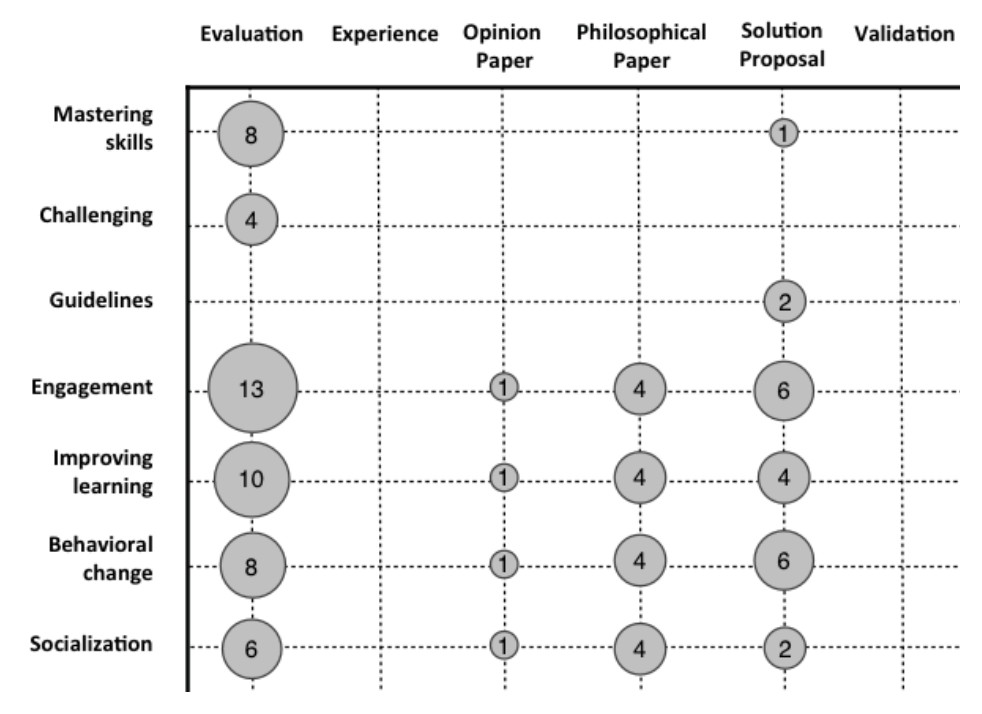
\includegraphics[width=.9\textwidth]{bubblemap_gamification}
\end{figure}

Table 6 also synthesizes the frequency of primary studies according
to research objective. The numbers in parenthesis represent the
number of papers in the category, while the numbers in square
brackets are the papers’ references. 24 of the 26 studies have
Engagement among students as their main objective. Only two
studies do not directly approach such an objective, discussing
motivation in a higher abstraction level. Contributing to further
improvement in how students socialize is mentioned by 13 studies
(Socialization). Nevertheless, only eight primary studies report
practical solutions to achieving such an objective, four encourage group activities, and one highlights the importance of this sort of
activity.

\textbf{Table 6. Distribution of gamification research by study type and research objectives}

A Venn diagram was drawn to clarify the distribution of the
overlapping studies (Figure 3). For simplicity’s sake, we decided to
include only four categories in the diagram. As shown in the
diagram, 9 papers overlap 4 research objectives. Some studies
encompass only two or three research objectives: (i) engagement
and behavioral change; (ii) socialization and engagement; and (iii)
improving learning, behavioral change, and engagement. This
suggests that motivating students is not a straightforward task that
can be accomplished by employing only one strategy. However, the
amount of studies that employ the four main research objectives
indicates that researchers have been striving to come up with more
sound solutions to motivate students.
Only one study mentions that computer-supported collaborative
learning (CSCL) is suited to develop applications that help students
to socialize and organize themselves in groups. However, this study
does not cover how to undertake the integration of computer-supported
collaborative learning, gamification, and educational
approaches. Therefore, the answer to RQ3 (What gamification
approaches have been most investigated in the field of CSCL?) is
that there is a lack of approaches that combine gamification and
computer-supported collaborative learning. 

\textbf{Figure 3. Overview of the four categories with the highest
number of papers and the overlap among them }

%---------------------------------------------
% Threats to Validity
%---------------------------------------------
\section{Threats to Validity}

In order to ensure an unbiased selection process, the RQs, inclusion
criteria, and exclusion criteria were established before the
conduction of the systematic mapping. Furthermore, the selection
process was carried out in an independent fashion by each involved
author. To mitigate any selection bias and improve validity, the
inclusion or exclusion of controversial studies was jointly decided.
Nevertheless, we cannot rule out threats from a quality assessment
perspective because during the selection process no scores were
assigned to studies.
Another threat to validity consists of whether we selected all
relevant studies in the area. Although such a threat cannot be ruled
out, we tried to mitigate it by taking into account several important
search engines. Therefore, we surmise that these search engines are
prone to contain the majority of the relevant studies. In the future,
we intend to update this scoping study by taking into account more
search engines. The coherency of our classification scheme also
represents a threat to the validity of this mapping study. As pointed
out by [27], one of the problems of mappings studies is how to
determine the proper way to categorize the resulting studies. 

%---------------------------------------------
% Concluding Remarks
%---------------------------------------------
\section{Concluding Remarks of the Systematic Mapping}

The main purpose of our mapping study is to provide an overview
of what has been investigated in the context of gamification applied
to education. To fulfill our goal, we followed a systematic
methodology, i.e., systematic mapping. We defined three research
questions to be answered by our mapping. RQ1: In what
educational contexts and levels has gamification been most
investigated? RQ2: What types of studies have been most
investigated in gamification and education? RQ3: What
gamification approaches have been most investigated in the field of
CSCL?
According to our results, most studies were published in
conferences and have focused on Higher Education (RQ1 – see
Table 2) to foster the engagement of students through learning
activities that build on gamification concepts (RQ2 – see Table 6).
We also identified that there is a lack of approaches that combine
gamification and CSCL (RQ3).
The novelty of this research is that, to the best of our
knowledge, this is the first systematic mapping covering research
into gamification applied to education. Another contribution of this
research is the map (Figure 2) we have created. By analyzing such
a map it is possible to identify in which way gamification has been
explored in educational contexts; thereby determining research
gaps and future research opportunities. 


\end{apendicesenv}
% ---

% ----------------------------------------------------------
% Anexos
% ----------------------------------------------------------

% ---
% Inicia os anexos
% ---
\begin{anexosenv}

%    \chapter{Gameful Design, Serious Games, video Games, and Gamification} 
%    \label{chapter:Game_related}
%    \begin{itemize}
\item Gamification is not Playful design or gameful design:
\end{itemize}

Playful design is using game-based aesthetics or limited usability
based on game elements in non-game contexts with the purpose of
drawing the user's attention \cite{Ferri2017}. These elements are used to amuse
users and cause an emotional response. One successful example is
Twitter’s page knows as “Fail Whale” (Figure~\ref{fig:failwhale}). Whenever
there is an overload on the servers, instead of a boring page with
some standard error message, users are presented with a drawing of
a dozen birds, twitters, trying to lift a whale \cite{kalbach2016mapping}.

% Playful design or gameful design
\begin{figure}[h!]
\caption{The (now retired) “Fail Whale” was used to illustrate Twitter's service outage.}
\centering

\includegraphics[width=0.4\textwidth]{failwhale}
\label{fig:failwhale}
\end{figure}

\begin{itemize}
\item Gamification is not Serious games:
\end{itemize}

Serious games are games designed for non-recreational
environments, however with learning and game objectives in focus \cite{Blanchard2011}. The term
“serious” is employed because these games can focus on areas as
diverse as economics, education, health, industry, military,
engineering, and politics. In environments created by applying
serious game concepts, it is possible to simulate real-world
situations without incurring in eventual costs and risks. The main
goal of this sort of training-environment is to convey information
to the user. The Virtual Incident Management Training System
(Figure~\ref{fig:serious_games}) is a multiplayer training environment designed for
training professionals that need to act swiftly in case of accident on
highways, such as paramedics and policemen \cite{catt_lab2017}.

% Serious game
\begin{figure}[h!]
\caption{The Virtual Incident Management Training System initial screen. Source: \cite{catt_lab2017}}
\centering
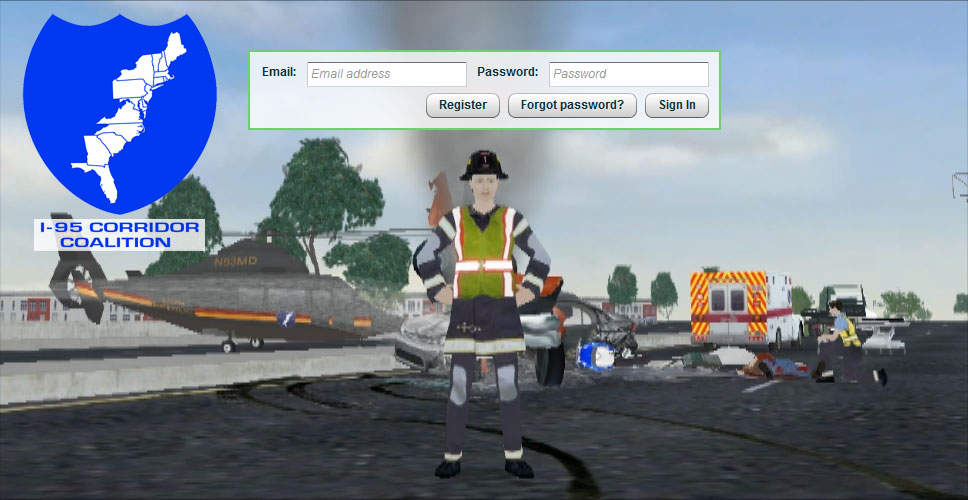
\includegraphics[width=0.5\textwidth]{serious_games}
\label{fig:serious_games}
\end{figure}

\begin{itemize}
\item Gamification is not video games or digital games:
\end{itemize}

Video Games or Digital Games are systems in which users are
engaged in resolving abstract conflicts and challenges, under
predetermined rules \cite{fullerton2008}. In this scenario the game continuously
offers interactivity and feedback to the user, which often result in
an emotional reaction. Figure 1-d shows a screenshot of the game
New Super Mario Bros.Wii\copyright whose main character, Mario, is
considered one of the most iconic video game characters.

% Video games or Digital games
\begin{figure}[h!]
\caption{New Super Mario Bros.wii a game developed and publishid by Nintendo}
\centering
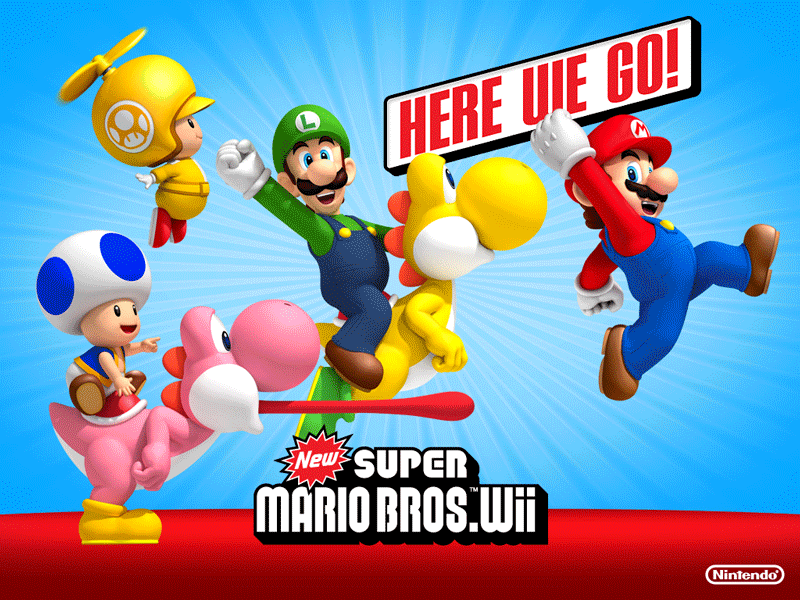
\includegraphics[width=0.4\textwidth]{super_mariowii}
\label{fig:super_mariowii}
\end{figure}


\end{anexosenv}
% ---

\end{document}